% !TeX spellcheck = de-DE
% !TeX encoding = utf8
% !TeX program = pdflatex
% !BIB program = biber
% -*- coding:utf-8 mod:LaTeX -*-

% vv  scroll down to line 200 for content  vv


\let\ifdeutsch\iftrue
\let\ifenglisch\iffalse
% EN: This file is loaded before the \documentclass command in the main document

% EN: The following package allows \\ at the title page
%     For more information see https://github.com/latextemplates/scientific-thesis-cover/issues/4
\RequirePackage{kvoptions-patch}

\ifenglisch
  \PassOptionsToClass{numbers=noenddot}{scrbook}
\else
  %()Aus scrguide.pdf - der Dokumentation von KOMA-Script)
  %Nach DUDEN steht in Gliederungen, in denen ausschließlich arabische Ziffern für die Nummerierung
  %verwendet werden, am Ende der Gliederungsnummern kein abschließender Punkt
  %(siehe [DUD96, R3]). Wird hingegen innerhalb der Gliederung auch mit römischen Zahlen
  %oder Groß- oder Kleinbuchstaben gearbeitet, so steht am Ende aller Gliederungsnummern ein
  %abschließender Punkt (siehe [DUD96, R4])
  \PassOptionsToClass{numbers=autoendperiod}{scrbook}
\fi

% Warns about outdated packages and missing caption declarations
% See https://www.ctan.org/pkg/nag
\RequirePackage[l2tabu, orthodox]{nag}

%DE: Neue deutsche Trennmuster
%    Siehe http://www.ctan.org/pkg/dehyph-exptl und http://projekte.dante.de/Trennmuster/WebHome
%    Nur für pdflatex, nicht für lualatex
\RequirePackage{ifluatex}
\ifluatex
  % do not load anything
\else
  \ifdeutsch
    \RequirePackage[ngerman=ngerman-x-latest]{hyphsubst}
  \fi
\fi

\documentclass[
  ngerman,
  % fontsize=11pt is the standard
  a4paper,  % Standard format - only KOMAScript uses paper=a4 - https://tex.stackexchange.com/a/61044/9075
  twoside,  % we are optimizing for both screen and two-side printing. So the page numbers will jump, but the content is configured to stay in the middle (by using the geometry package)
  bibliography=totoc,
  %               idxtotoc,   %Index ins Inhaltsverzeichnis
  %               liststotoc, %List of X ins Inhaltsverzeichnis, mit liststotocnumbered werden die Abbildungsverzeichnisse nummeriert
  headsepline,
  cleardoublepage=empty,
  parskip=half,
  %               draft    % um zu sehen, wo noch nachgebessert werden muss - wichtig, da Bindungskorrektur mit drin
  draft=false
]{scrbook}
% !TeX encoding = utf8
% -*- coding:utf-8 mod:LaTeX -*-

% EN: This file includes basic packages and sets options. The order of package
%     loading is important

% DE: In dieser Datei werden zuerst die benoetigten Pakete eingebunden und
%     danach diverse Optionen gesetzt. Achtung Reihenfolge ist entscheidend!


% EN: Styleguide:
% - English comments are prefixed with "EN", German comments are prefixed with "DE"
% - Prefixed headings define the language for the subsequent paragraphs
% - It is tried to organize packages in blocks. Bocks are separated by two empty lines.

% DE: Styleguide:
%
% Ein sehr kleiner Styleguide. Packages werden in Blöcken organisiert.
% Zwischen zwei Blöcken sind 2 Leerzeilen!


% EN: Enable copy and paste of text from the PDF
%     Only required for pdflatex. It "just works" in the case of lualatex.
%     mmap enables mathematical symbols, but does not work with the newtx font set
%     See: https://tex.stackexchange.com/a/64457/9075
%     Other solutions outlined at http://goemonx.blogspot.de/2012/01/pdflatex-ligaturen-und-copynpaste.html and http://tex.stackexchange.com/questions/4397/make-ligatures-in-linux-libertine-copyable-and-searchable
%     Trouble shooting outlined at https://tex.stackexchange.com/a/100618/9075

\ifluatex
\else
  \usepackage{cmap}
\fi


% EN: File encoding
% DE: Codierung
%     Wir sind im 21 Jahrhundert, utf-8 löst so viele Probleme.
%
% Mit UTF-8 funktionieren folgende Pakete nicht mehr. Bitte beachten!
%   * fancyvrb mit §
%   * easylist -> http://www.ctan.org/tex-archive/macros/latex/contrib/easylist/
\ifluatex
  % EN: See https://tex.stackexchange.com/a/158517/9075
  %     Not required, because of usage of fontspec package
  %\usepackage[utf8]{luainputenc}
\else
  \usepackage[utf8]{inputenc}
\fi


% DE: Parallelbetrieb tex4ht und pdflatex

\makeatletter
\@ifpackageloaded{tex4ht}{
  \def\iftex4ht{\iftrue}
}{
  \def\iftex4ht{\iffalse}
}
\makeatother


% EN: Mathematics
% DE: Mathematik
%
% DE: Viele Mathematik-Sachen. Siehe https://texdoc.net/pkg/amsmath
%
% EN: Options must be passed this way, otherwise it does not work with glossaries
% DE: fleqn (=Gleichungen linksbündig platzieren) funktioniert nicht direkt. Es muss noch ein Patch gemacht werden:
\PassOptionsToPackage{fleqn,leqno}{amsmath}
%
% DE: amsmath Muss nicht mehr geladen werden, da es von newtxmath automatisch geladen wird
% \usepackage{amsmath}


%% EN: Fonts
%% DE: Schriften
%%
%% !!! If you change the font, be sure that words such as "workflow" can
%% !!! still be copied from the PDF. If this is not the case, you have
%% !!! to use glyphtounicode. See comment at cmap package


% EN: Times Roman for all text
\ifluatex
  \RequirePackage{amsmath}
  \RequirePackage{unicode-math}
  \setmainfont{TeX Gyre Termes}
  \setmathfont{texgyretermes-math.otf}
  \setsansfont[Scale=.9]{TeX Gyre Heros}
  \setmonofont[StylisticSet={1,3},Scale=.9]{inconsolata}
\else
  \RequirePackage{newtxtext}
  \RequirePackage{newtxmath}
  % EN: looks good with times, but no equivalent for lualatex found,
  %     therefore replaced with inconsolata
  %\RequirePackage[zerostyle=b,scaled=.9]{newtxtt}
  \RequirePackage[varl,scaled=.9]{inconsolata}

  % DE: Symbole
  % unicode-math scheint für die meisten schon etwas anzubieten
  %
  %\usepackage[geometry]{ifsym} % \BigSquare

  % EN: The euro sign
  % DE: Das Euro Zeichen
  %     Fuer Palatino (mathpazo.sty): richtiges Euro-Zeichen
  %     Alternative: \usepackage{eurosym}
  \newcommand{\EUR}{\ppleuro}
\fi


% DE: Noch mehr Symbole
%\usepackage{stmaryrd} %fuer \ovee, \owedge, \otimes
%\usepackage{marvosym} %fuer \Writinghand %patched to not redefine \Rightarrow
%\usepackage{mathrsfs} %mittels \mathscr{} schoenen geschwungenen Buchstaben erzeugen
%\usepackage{calrsfs} %\mathcal{} ein bisserl dickeren buchstaben erzeugen - sieht net so gut aus.

% EN: Fallback font - if the subsequent font packages do not define a font (e.g., monospaced)
%     This is the modern package for "Computer Modern".
%     In case this gets activated, one has to switch from cmap package to glyphtounicode (in the case of pdflatex)
% DE: Fallback-Schriftart
%\usepackage[%
%    rm={oldstyle=false,proportional=true},%
%    sf={oldstyle=false,proportional=true},%
%    tt={oldstyle=false,proportional=true,variable=true},%
%    qt=false%
%]{cfr-lm}

% EN: Headings are typset in Helvetica (which is similar to Arial)
% DE: Schriftart fuer die Ueberschriften - ueberschreibt lmodern
%\usepackage[scaled=.95]{helvet}

% DE: Für Schreibschrift würde tun, muss aber nicht
%\usepackage{mathrsfs} %  \mathscr{ABC}

% EN: Font for the main text
% DE: Schriftart fuer den Fliesstext - ueberschreibt lmodern
%     Linux Libertine, siehe http://www.linuxlibertine.org/
%     Packageparamter [osf] = Minuskel-Ziffern
%     rm = libertine im Brottext, Linux Biolinum NICHT als serifenlose Schrift, sondern helvet (von oben) beibehalten
%\usepackage[rm]{libertine}

% EN: Alternative Font: Palantino. It is recommeded by Prof. Ludewig for German texts
% DE: Alternative Schriftart: Palantino, Packageparamter [osf] = Minuskel-Ziffern
%     Bitte nur in deutschen Texten
%\usepackage{mathpazo} %ftp://ftp.dante.de/tex-archive/fonts/mathpazo/ - Tipp aus DE-TEX-FAQ 8.2.1

% DE: Schriftart fuer Programmcode - ueberschreibt lmodern
%     Falls auskommentiert, wird die Standardschriftart lmodern genommen
%     Fuer schreibmaschinenartige Schluesselwoerter in den Listings - geht bei alten Installationen nicht, da einige Fontshapes (<>=) fehlen
%\usepackage[scaled=.92]{luximono}
%\usepackage{courier}
% DE: BeraMono als Typewriter-Schrift, Tipp von http://tex.stackexchange.com/a/71346/9075
%\usepackage[scaled=0.83]{beramono}

% EN: backticks (`) are rendered as such in verbatim environments.
%     See following links for details:
%     - https://tex.stackexchange.com/a/341057/9075
%     - https://tex.stackexchange.com/a/47451/9075
%     - https://tex.stackexchange.com/a/166791/9075
\usepackage{upquote}

% EN: For \texttrademark{}
\usepackage{textcomp}

% EN: name-clashes von marvosym und mathabx vermeiden:
\def\delsym#1{%
  %  \expandafter\let\expandafter\origsym\expandafter=\csname#1\endcsname
  %  \expandafter\let\csname orig#1\endcsname=\origsym
  \expandafter\let\csname#1\endcsname=\relax
}

%\usepackage{pifont}
%\usepackage{bbding}
%\delsym{Asterisk}
%\delsym{Sun}\delsym{Mercury}\delsym{Venus}\delsym{Earth}\delsym{Mars}
%\delsym{Jupiter}\delsym{Saturn}\delsym{Uranus}\delsym{Neptune}
%\delsym{Pluto}\delsym{Aries}\delsym{Taurus}\delsym{Gemini}
%\delsym{Rightarrow}
%\usepackage{mathabx} - Ueberschreibt leider zu viel - und die \le-Zeichen usw. sehen nicht gut aus!


% EN: Modern font encoding
%     Has to be loaded AFTER any font packages. See https://tex.stackexchange.com/a/2869/9075.
\ifluatex
\else
  \usepackage[T1]{fontenc}
\fi
%


% EN: Character protrusion and font expansion. See http://www.ctan.org/tex-archive/macros/latex/contrib/microtype/
% DE: Optischer Randausgleich und Grauwertkorrektur

\usepackage[
  babel=true, % EN: Enable language-specific kerning. Take language-settings from the languge of the current document (see Section 6 of microtype.pdf)
  expansion=alltext,
  protrusion=alltext-nott, % EN: Ensure that at listings, there is no change at the margin of the listing
  final % EN: Always enable microtype, even if in draft mode. This helps finding bad boxes quickly.
        %     In the standard configuration, this template is always in the final mode, so this option only makes a difference if "pros" use the draft mode
]{microtype}


% EN: \texttt{test -- test} keeps the "--" as "--" (and does not convert it to an en dash)
\DisableLigatures{encoding = T1, family = tt* }

% DE: fuer microtype
% DE: tracking=true muss als Parameter des microtype-packages mitgegeben werden
% DE: Deaktiviert, da dies bei Algorithmen seltsam aussieht

%\DeclareMicrotypeSet*[tracking]{my}{ font = */*/*/sc/* }%
%\SetTracking{ encoding = *, shape = sc }{ 45 }
% DE: Hier wird festgelegt,
%     dass alle Passagen in Kapitälchen automatisch leicht
%     gesperrt werden.
%     Quelle: http://homepage.ruhr-uni-bochum.de/Georg.Verweyen/pakete.html
%    Deaktiviert, da sonst "BPEL", "BPMN" usw. wirklich komisch aussehen.
%     Macht wohl nur bei geisteswissenschaftlichen Arbeiten Sinn.


% EN: amsmath teaks


% EN: Fixes bugs in AMS math
%     Corrently conflicts with unicode-math
% \usepackage{mathtools}

%\numberwithin{equation}{section}
%\renewcommand{\theequation}{\thesection.\Roman{equation}}

% EN: work-around ams-math problem with align and 9 -> 10. Does not work with glossaries, No visual changes.
%\addtolength\mathindent{1em}


% EN: For theorems, replacement for amsthm
\usepackage[amsmath,hyperref]{ntheorem}
\theorempreskipamount 2ex plus1ex minus0.5ex
\theorempostskipamount 2ex plus1ex minus0.5ex
\theoremstyle{break}
\newtheorem{definition}{Definition}[section]


% CTAN: https://ctan.org/pkg/lccaps
% Doc: http://texdoc.net/pkg/lccaps
%
% Required for DE/EN \initialism
\usepackage{lccaps}


% EN: Defintion of colors. Argument "hyperref" is not used as we do not want to change border colors of links: Links are not colored anymore.
% DE: Farbdefinitionen
\usepackage[dvipsnames]{xcolor}


% EN: Required for custom acronyms/glossaries style.
%     Left aligned Columns in tables with fixed width.
%     See http://tex.stackexchange.com/questions/91566/syntax-similar-to-centering-for-right-and-left
\usepackage{ragged2e}


% DE: Wichtig, ansonsten erscheint "No room for a new \write"
\usepackage{scrwfile}


% EN: Support for language-specific hyphenation
% DE: Neue deutsche Rechtschreibung und Literatur statt "Literature"
%     Die folgende Einstellung ist der Nachfolger von ngerman.sty
\ifdeutsch
  % DE: letzte Sprache ist default, Einbindung von "american" ermöglicht \begin{otherlanguage}{amercian}...\end{otherlanguage} oder \foreignlanguage{american}{Text in American}
  %     Siehe auch http://tex.stackexchange.com/a/50638/9075
  \usepackage[american,main=ngerman]{babel}
  % Ein "abstract" ist eine "Kurzfassung", keine "Zusammenfassung"
  \addto\captionsngerman{%
    \renewcommand\abstractname{Kurzfassung}%
  }
  \ifluatex
    % EN: conditionally disable ligatures. See https://github.com/latextemplates/scientific-thesis-template/issues/54
    %     for a discussion
    \usepackage[ngerman]{selnolig}
  \fi
\else
  % EN: Set English as language and allow to write hyphenated"=words
  %     `american`, `english` and `USenglish` are synonyms for babel package (according to https://tex.stackexchange.com/questions/12775/babel-english-american-usenglish).
  %      "english" has to go last to set it as default language
  \usepackage[ngerman,main=english]{babel}
  % EN: Hint by http://tex.stackexchange.com/a/321066/9075 -> enable "= as dashes
  \addto\extrasenglish{\languageshorthands{ngerman}\useshorthands{"}}
  \ifluatex
    % EN: conditionally disable ligatures. See https://github.com/latextemplates/scientific-thesis-template/issues/54
    %     for a discussion
    \usepackage[english]{selnolig}
  \fi
\fi
%


% EN: For easy quotations: \enquote{text}
%     This package is very smart when nesting is applied, otherwise textcmds (see below) provides a shorter command
%     Note that this package results in a warning when it is loaded before minted (actually fvextra).
% DE: Anführungszeichen
%     Zitate in \enquote{...} setzen, dann werden automatisch die richtigen Anführungszeichen verwendet.
%     Dieses package erzeugt eine Warnung, wenn es vor minted (genauer fvextra) geladen wird.
\usepackage{csquotes}


% EN: For even easier quotations: \qq{text}.
%     Is not smart in the case of nesting, but good enough for the most cases
\usepackage{textcmds}
\ifdeutsch
  % EN: German quotes are different. So do not use the English quotes, but the ones provided by the csquotes package.
  \renewcommand{\qq}[1]{\enquote{#1}}
\fi


% EN: extended enumarations
% DE: erweitertes Enumerate
\usepackage{paralist}


% DE: Gestaltung der Kopf- und Fußteilen

\usepackage[automark]{scrlayer-scrpage}

\automark[section]{chapter}
\setkomafont{pageheadfoot}{\normalfont\sffamily}
\setkomafont{pagenumber}{\normalfont\sffamily}

% DE: funktioniert nicht: Alle Linien sind hier weg
%\setheadsepline[.4pt]{.4pt}


% DE: Intelligentes Leerzeichen um hinter Abkürzungen die richtigen Abstände zu erhalten, auch leere.
%     Siehe commands.tex \gq{}
\usepackage{xspace}
% DE: Macht \xspace und \enquote kompatibel
\makeatletter
\xspaceaddexceptions{\grqq \grq \csq@qclose@i \} }
\makeatother


\newcommand{\eg}{e.\,g.,\ }
\newcommand{\ie}{i.\,e.,\ }


% EN: introduce \powerset - hint by http://matheplanet.com/matheplanet/nuke/html/viewtopic.php?topic=136492&post_id=997377
\DeclareFontFamily{U}{MnSymbolC}{}
\DeclareSymbolFont{MnSyC}{U}{MnSymbolC}{m}{n}
\DeclareFontShape{U}{MnSymbolC}{m}{n}{
  <-6>    MnSymbolC5
  <6-7>   MnSymbolC6
  <7-8>   MnSymbolC7
  <8-9>   MnSymbolC8
  <9-10>  MnSymbolC9
  <10-12> MnSymbolC10
  <12->   MnSymbolC12%
}{}
\DeclareMathSymbol{\powerset}{\mathord}{MnSyC}{180}


% EN: Package for the appendix
% DE: Anhang
\usepackage{appendix}
%[toc,page,title,header]
%


% EN: Graphics
% DE: Grafikeinbindungen
%
% EN: The parameter "pdftex" is not required
\usepackage{graphicx}
\graphicspath{{\getgraphicspath}}
\newcommand{\getgraphicspath}{graphics/}


% EN: Enables inclusion of SVG graphics - 1:1 approach
%    This is NOT the approach of https://ctan.org/pkg/svg-inkscape,
%     which allows text in SVG to be typeset using LaTeX
%     We just include the SVG as is.
\usepackage{epstopdf}
\epstopdfDeclareGraphicsRule{.svg}{pdf}{.pdf}{%
  inkscape -z -D --file=#1 --export-pdf=\OutputFile
}


% EN: Enables inclusion of SVG graphics - text-rendered-with-LaTeX-approach
%     This is the approach of https://ctan.org/pkg/svg-inkscape,
\newcommand{\executeiffilenewer}[3]{%
  \IfFileExists{#2}
  {
    %\message{file #2 exists}
    \ifnum\pdfstrcmp{\pdffilemoddate{#1}}%
      {\pdffilemoddate{#2}}>0%
      {\immediate\write18{#3}}
    \else
      {%\message{file up to date #2}
      }
    \fi%
  }{
    %\message{file #2 doesn't exist}
    %\message{argument: #3}
    %\immediate\write18{echo "test" > xoutput.txt}
    \immediate\write18{#3}
  }
}
\newcommand{\includesvg}[1]{%
  \executeiffilenewer{#1.svg}{#1.pdf}%
  {
    inkscape -z -D --file=\getgraphicspath#1.svg %
    --export-pdf=\getgraphicspath#1.pdf --export-latex}%
  \input{\getgraphicspath#1.pdf_tex}%
}


% EN: Enable typesetting values with SI units.
\ifdeutsch
  \usepackage[mode=text,group-minimum-digits=4]{siunitx}
  \sisetup{locale=DE}
\else
  \usepackage[mode=text,group-minimum-digits=4,group-separator={,}]{siunitx}
  \sisetup{locale=US}
\fi


% EN: Extensions for tables
% DE: Tabellenerweiterungen
\usepackage{array} %increases tex's buffer size and enables ``>'' in tablespecs
\usepackage{longtable}
\usepackage{dcolumn} %Aligning numbers by decimal points in table columns
\ifdeutsch
  \newcolumntype{d}[1]{D{.}{,}{#1}}
\else
  \newcolumntype{d}[1]{D{.}{.}{#1}}
\fi
\setlength{\extrarowheight}{1pt}


% DE: Eine Zelle, die sich über mehrere Zeilen erstreckt.
%     Siehe Beispieltabelle in Kapitel 2
\usepackage{multirow}


% DE: Fuer Tabellen mit Variablen Spaltenbreiten
%\usepackage{tabularx}
%\usepackage{tabulary}


% EN: Links behave as they should. Enables "\url{...}" for URL typesettings.
%     Allow URL breaks also at a hyphen, even though it might be confusing: Is the "-" part of the address or just a hyphen?
%     See https://tex.stackexchange.com/a/3034/9075.
% DE: Links verhalten sich so, wie sie sollen
%     Zeilenumbrüche bei URLs auch bei Bindestrichen erlauben, auch wenn es verwirrend sein könnte: Gehört der Bindestrich zur URL oder ist es ein Trennstrich?
%     Siehe https://tex.stackexchange.com/a/3034/9075.
\usepackage[hyphens]{url}
%
%  EN: When activated, use text font as url font, not the monospaced one.
%      For all options see https://tex.stackexchange.com/a/261435/9075.
% \urlstyle{same}
%
% EN: Hint by http://tex.stackexchange.com/a/10419/9075.
\makeatletter
\g@addto@macro{\UrlBreaks}{\UrlOrds}
\makeatother


% DE: Index über Begriffe, Abkürzungen
%\usepackage{makeidx} makeidx ist out -> http://xindy.sf.net verwenden


% DE: lustiger Hack fuer das Abkuerzungsverzeichnis
%     nach latex durchlauf folgendes ausfuehren
%     makeindex ausarbeitung.nlo -s nomencl.ist -o ausarbeitung.nls
%     danach nochmal latex
%\usepackage{nomencl}
%    \let\abk\nomenclature %Deutsche Ueberschrift setzen
%          \renewcommand{\nomname}{List of Abbreviations}
%        %Punkte zw. Abkuerzung und Erklaerung
%          \setlength{\nomlabelwidth}{.2\hsize}
%          \renewcommand{\nomlabel}[1]{#1 \dotfill}
%        %Zeilenabstaende verkleinern
%          \setlength{\nomitemsep}{-\parsep}
%    \makenomenclature


% EN: Logic for TeX - enables if-then-else in commands
% DE: Logik für TeX
%     FÜr if-then-else @ commands.tex
\usepackage{ifthen}


% EN: Code Listings
% DE: Listings
\usepackage{listings}
\lstset{language=XML,
  showstringspaces=false,
  extendedchars=true,
  basicstyle=\footnotesize\ttfamily,
  commentstyle=\slshape,
  % DE: Original: \rmfamily, damit werden die Strings im Quellcode hervorgehoben. Zusaetzlich evtl.: \scshape oder \rmfamily durch \ttfamily ersetzen. Dann sieht's aus, wie bei fancyvrb
  stringstyle=\ttfamily,
  breaklines=true,
  breakatwhitespace=true,
  % EN: alternative: fixed
  columns=flexible,
  numbers=left,
  numberstyle=\tiny,
  basewidth=.5em,
  xleftmargin=.5cm,
  % aboveskip=0mm, %DE: deaktivieren, falls man lstlistings direkt als floating object benutzt (\begin{lstlisting}[float,...])
  % belowskip=0mm, %DE: deaktivieren, falls man lstlistings direkt als floating object benutzt (\begin{lstlisting}[float,...])
  captionpos=b
}

\ifluatex
\else
  % EN: Enable UTF-8 support - see https://tex.stackexchange.com/q/419327/9075
  \usepackage{listingsutf8}
  \lstset{inputencoding=utf8/latin1}
\fi

\ifdeutsch
  \renewcommand{\lstlistlistingname}{Verzeichnis der Listings}
\fi


% EN: Alternative to listings could be fancyvrb. Can be used together.
% DE: Alternative zu Listings ist fancyvrb. Kann auch beides gleichzeitig benutzt werden.
\usepackage{fancyvrb}
%
% EN: Font size for the normal text
% DE: Groesse fuer den Fliesstext. Falls deaktiviert: \normalsize
%\fvset{fontsize=\small}
%
% DE: Somit kann im Text ganz einfach §verbatim§ text gesetzt werden.
%     Disabled, because UTF-8 does not work any more and lualatex causes issues
%\DefineShortVerb{\§}
%
% EN: Shrink font size of listings
\RecustomVerbatimEnvironment{Verbatim}{Verbatim}{fontsize=\footnotesize}
\RecustomVerbatimCommand{\VerbatimInput}{VerbatimInput}{fontsize=\footnotesize}
%
% EN: Hack for fancyvrb based on http://newsgroups.derkeiler.com/Archive/Comp/comp.text.tex/2008-12/msg00075.html
%     Change of the solution: \Vref somehow collidated with cleveref/varioref as the output of \Vref{} was "Abschnitt 4.3 auf Seite 85"; therefore changed to \myVref -- so completely removed
%     See https://tex.stackexchange.com/q/132420/9075 for more information.
\newcommand{\Vlabel}[1]{\label[line]{#1}\hypertarget{#1}{}}
\newcommand{\lref}[1]{\hyperlink{#1}{\FancyVerbLineautorefname~\ref*{#1}}}


% EN: Tunings of captions for floats, listings, ...
% DE: Bildunterschriften bei floats genauso formatieren wie bei Listings
%     Anpassung wird unten bei den newfloat-Deklarationen vorgenommen
%     https://www.ctan.org/pkg/caption2 is superseeded by this package.
\usepackage{caption}


% EN: Provides rotating figures, where the PDF page is also turned
% DE: Ermoeglicht es, Abbildungen um 90 Grad zu drehen
%     Alternatives Paket: rotating Allerdings wird hier nur das Bild gedreht, während bei lscape auch die PDF-Seite gedreht wird.
%     Das Paket lscape dreht die Seite auch nicht
\usepackage{pdflscape}


% EN: Required for proper environments of fancyvrb and lstlistings
%    There is also the newfloat pacakge (recommended by minted), but we currently have no expericene with that
% DE: Wird für fancyvrb und für lstlistings verwendet
\usepackage{float}
%
% EN: Alternative to float package
%\usepackage{floatrow}
% DE: zustäzlich für den Paramter [H] = Floats WIRKLICH da wo sie deklariert wurden paltzieren - ganz ohne Kompromisse
%     floatrow ist der Nachfolger von float
%     Allerdings macht floatrow in manchen Konstellationen Probleme. Deshalb ist das Paket deaktiviert.
%
% EN: See http://www.tex.ac.uk/cgi-bin/texfaq2html?label=floats
% DE: floats IMMER nach einer Referenzierung platzieren
%\usepackage{flafter}


% EN: Put footnotes below floats
%     Source: https://tex.stackexchange.com/a/32993/9075
\usepackage{stfloats}
\fnbelowfloat


% EN: For nested figures
% DE: Fuer Abbildungen innerhalb von Abbildungen
%     Ersetzt die Pakete subfigure und subfig - siehe https://tex.stackexchange.com/a/13778/9075
\usepackage[hypcap=true]{subcaption}


% EN: Extended support for footnotes
% DE: Fußnoten
%
%\usepackage{dblfnote}  %Zweispaltige Fußnoten
%
% Keine hochgestellten Ziffern in der Fußnote (KOMA-Script-spezifisch):
%\deffootnote[1.5em]{0pt}{1em}{\makebox[1.5em][l]{\bfseries\thefootnotemark}}
%
% Abstand zwischen Fußnoten vergrößern:
%\setlength{\footnotesep}{.85\baselineskip}
%
% EN: Following command disables the separting line of the footnote
% DE: Folgendes Kommando deaktiviert die Trennlinie zur Fußnote
%\renewcommand{\footnoterule}{}
%
\addtolength{\skip\footins}{\baselineskip} % Abstand Text <-> Fußnote
%
% Fußnoten immer ganz unten auf einer \raggedbottom-Seite
% fnpos kommt aus dem yafoot package
\usepackage{fnpos}
\makeFNbelow
\makeFNbottom


% EN: Variable page heights
% DE: Variable Seitenhöhen zulassen
\raggedbottom


% DE: Falls die Seitenzahl bei einer Referenz auf eine Abbildung nur dann angegeben werden soll,
%     falls sich die Abbildung nicht auf der selben Seite befindet...
\iftex4ht
  %tex4ht does not work well with vref, therefore we emulate vref behavior
  \newcommand{\vref}[1]{\ref{#1}}
\else
  \ifdeutsch
    \usepackage[ngerman]{varioref}
  \else
    \usepackage{varioref}
  \fi
\fi


% EN: More beautiful tables if one uses \toprule, \midrule, \bottomrule
% DE: Noch schoenere Tabellen als mit booktabs mit http://www.zvisionwelt.de/downloads.html
\usepackage{booktabs}
%
%\usepackage[section]{placeins}


% EN: Graphs and Automata
%
% TODO: Since version 3.0 (2013-10-01), it supports pdflatex via the auto-pst-pdf package
%       Requires -shell-escape
%\usepackage{gastex}


%\usepackage{multicol}

% DE: kollidiert mit diplomarbeit.sty
%\usepackage{setspace}


% DE: biblatex statt bibtex
\usepackage[
  backend       = biber, %biber does not work with 64x versions alternative: bibtex8
  %minalphanames only works with biber backend
  sortcites     = true,
  bibstyle      = alphabetic,
  citestyle     = alphabetic,
  giveninits    = true,
  useprefix     = false, %"von, van, etc." will be printed, too. See below.
  minnames      = 1,
  minalphanames = 3,
  maxalphanames = 4,
  maxbibnames   = 99,
  maxcitenames  = 2,
  natbib        = true,
  eprint        = true,
  url           = true,
  doi           = true,
  isbn          = true,
  backref       = true]{biblatex}

% enable more breaks at URLs. See https://tex.stackexchange.com/a/134281.
\setcounter{biburllcpenalty}{7000}
\setcounter{biburlucpenalty}{8000}

\bibliography{bibliography}
%\addbibresource[datatype=bibtex]{bibliography.bib}

%Do not put "vd" in the label, but put it at "\citeauthor"
%Source: http://tex.stackexchange.com/a/30277/9075
\makeatletter
\AtBeginDocument{\toggletrue{blx@useprefix}}
\AtBeginBibliography{\togglefalse{blx@useprefix}}
\makeatother

%Thin spaces between initials
%http://tex.stackexchange.com/a/11083/9075
\renewrobustcmd*{\bibinitdelim}{\,}

%Keep first and last name together in the bibliography
%http://tex.stackexchange.com/a/196192/9075
\renewcommand*\bibnamedelimc{\addnbspace}
\renewcommand*\bibnamedelimd{\addnbspace}

%Replace last "and" by comma in bibliography
%See http://tex.stackexchange.com/a/41532/9075
\AtBeginBibliography{%
  \renewcommand*{\finalnamedelim}{\addcomma\space}%
}

\DefineBibliographyStrings{ngerman}{
  backrefpage  = {zitiert auf S\adddot},
  backrefpages = {zitiert auf S\adddot},
  andothers    = {et\ \addabbrvspace al\adddot},
  %Tipp von http://www.mrunix.de/forums/showthread.php?64665-biblatex-Kann-%DCberschrift-vom-Inhaltsverzeichnis-nicht-%E4ndern&p=293656&viewfull=1#post293656
  bibliography = {Literaturverzeichnis}
}

% EN: enable hyperlinked author names when using \citeauthor
%     source: http://tex.stackexchange.com/a/75916/9075
\DeclareCiteCommand{\citeauthor}
{\boolfalse{citetracker}%
  \boolfalse{pagetracker}%
  \usebibmacro{prenote}}
{\ifciteindex
  {\indexnames{labelname}}
  {}%
  \printtext[bibhyperref]{\printnames{labelname}}}
{\multicitedelim}
{\usebibmacro{postnote}}

% EN: natbib compatibility
%\newcommand{\citep}[1]{\cite{#1}}
%\newcommand{\citet}[1]{\citeauthor{#1} \cite{#1}}
% EN: Beginning of sentence - analogous to cleveref - important for names such as "zur Muehlen"
%\newcommand{\Citep}[1]{\cite{#1}}
%\newcommand{\Citet}[1]{\Citeauthor{#1} \cite{#1}}

% DE: Blindtext. Paket "blindtext" ist fortgeschritterner als "lipsum" und kann auch Mathematik im Text (http://texblog.org/2011/02/26/generating-dummy-textblindtext-with-latex-for-testing/)
%     kantlipsum (https://www.ctan.org/tex-archive/macros/latex/contrib/kantlipsum) ist auch ganz nett, aber eben auch keine Mathematik
%     Wird verwendet, um etwas Text zu erzeugen, um eine volle Seite wegen Layout zu sehen.
\usepackage[math]{blindtext}


% EN: Make LaTeX logos available by commands. E.g., \lualatex
%     Disabled, because currently causes \not= already defined
%\usepackage{dtk-logos}

% quick replacement:
\newcommand{\LuaLaTeX}{Lua\LaTeX\xspace}
\newcommand{\lualatex}{\LuaLaTeX}

% DE: Neue Pakete bitte VOR hyperref einbinden. Insbesondere bei Verwendung des
%     Pakets "index" wichtig, da sonst die Referenzierung nicht funktioniert.
%     Für die Indizierung selbst ist unter http://xindy.sourceforge.net
%     ein gutes Tool zu erhalten.
%     Hier also neue packages einbinden.
% EN: Add new packages at this place.


% EN: Provides hyperlinks
%     Option "unicode" fixes umlauts in the PDF bookmarks - see https://tex.stackexchange.com/a/338770/9075
%
% DE: Erlaubt Hyperlinks im Dokument.
%     Alle Optionen nach \hypersetup verschoben, sonst crash
%     Siehe auch: "Praktisches LaTeX" - www.itp.uni-hannover.de/~kreutzm
\usepackage[unicode]{hyperref}


% EN: Define colors
% DE: Da es mit KOMA 3 und xcolor zu Problemen mit den global Options kommt MÜSSEN die Optionen so gesetzt werden.
%     Eigene Farbdefinitionen ohne die Namen des xcolor packages
\definecolor{darkblue}{rgb}{0,0,.5}
\definecolor{black}{rgb}{0,0,0}


% EN: Define color of links and more
\hypersetup{
  % have both title and number hyperlinking to content
  linktoc=all,
  bookmarksnumbered=true,
  bookmarksopen=true,
  bookmarksopenlevel=1,
  breaklinks=true,
  colorlinks=true,
  pdfstartview=Fit,
  pdfpagelayout=SinglePage, % DE: Alterntaive: TwoPageRight -- zweiseitige Darstellung: ungerade Seiten rechts im PDF-Viewer - siehe auch http://tex.stackexchange.com/a/21109/9075
  %pdfencoding=utf8, % EN: This is probably the same as passing the option "unicode" at \usepackage{hyperref}
  filecolor=darkblue,
  urlcolor=darkblue,
  linkcolor=black,
  citecolor=black
}


% EN: Abbreviations - has to be loaded after hyperref
% DE: Abkürzungsverzeichnis - muss nach hyperref geladen werden
%
% DE: siehe http://www.dickimaw-books.com/cgi-bin/faq.cgi?action=view&categorylabel=glossaries#glsnewwriteexceeded
\usepackage[acronym,indexonlyfirst,nomain]{glossaries}
\ifdeutsch
  \addto\captionsngerman % DE: siehe https://tex.stackexchange.com/a/154566
  {%
    \renewcommand*{\acronymname}{Abkürzungsverzeichnis}
  }
\else
  \renewcommand*{\acronymname}{List of Abbreviations}
\fi
\renewcommand*{\glsgroupskip}{}
%
% EN: Removed Glossarie as a table as a quick fix to get the template working again
%     See http://tex.stackexchange.com/questions/145579/how-to-print-acronyms-of-glossaries-into-a-table
%
\makenoidxglossaries


% EN: Extensions for references inside the document (\cref{fig:sample}, ...)
% DE: cleveref für cref statt autoref, da cleveref auch bei Definitionen funktioniert
\usepackage[capitalise,nameinlink,noabbrev]{cleveref}
\ifdeutsch
  \crefname{table}{Tabelle}{Tabellen}
  \Crefname{table}{Tabelle}{Tabellen}
  \crefname{figure}{\figurename}{\figurename}
  \Crefname{figure}{Abbildung}{Abbildungen}
  \crefname{equation}{Gleichung}{Gleichungen}
  \Crefname{equation}{Gleichung}{Gleichungen}
  \crefname{theorem}{Theorem}{Theoreme}
  \Crefname{theorem}{Theorem}{Theoreme}
  \crefname{listing}{\lstlistingname}{\lstlistingname}
  \Crefname{listing}{Listing}{Listings}
  \crefname{section}{Abschnitt}{Abschnitte}
  \Crefname{section}{Abschnitt}{Abschnitte}
  \crefname{paragraph}{Abschnitt}{Abschnitte}
  \Crefname{paragraph}{Abschnitt}{Abschnitte}
  \crefname{subparagraph}{Abschnitt}{Abschnitte}
  \Crefname{subparagraph}{Abschnitt}{Abschnitte}
\else
  \crefname{listing}{\lstlistingname}{\lstlistingname}
  \Crefname{listing}{Listing}{Listings}
\fi


% DE: Zur Darstellung von Algorithmen
%     Algorithm muss nach hyperref geladen werden
\usepackage[chapter]{algorithm}
\usepackage[]{algpseudocode}


% DE: Links auf Gleitumgebungen springen nicht zur Beschriftung,
%     Doc: http://mirror.ctan.org/tex-archive/macros/latex/contrib/oberdiek/hypcap.pdf
%     sondern zum Anfang der Gleitumgebung
\usepackage[all]{hypcap}


% DE: Deckblattstyle
%
\ifdeutsch
  \PassOptionsToPackage{language=german}{scientific-thesis-cover}
\else
  \PassOptionsToPackage{language=english}{scientific-thesis-cover}
\fi


% EN: Bugfixes packages
%\usepackage{fixltx2e} %Fuer neueste LaTeX-Installationen nicht mehr benoetigt - bereinigte einige Ungereimtheiten, die auf Grund von Rueckwaertskompatibilitaet beibahlten wurden.
%\usepackage{mparhack} %Fixt die Position von marginpars (die in DAs selten bis gar nicht gebraucht werden}
%\usepackage{ellipsis} %Fixt die Abstaende vor \ldots. Wird wohl auch nicht benoetigt.


% EN: Settings for captions of floats
% DE: Formatierung der Beschriftungen
%
\captionsetup{
  format=hang,
  labelfont=bf,
  justification=justified,
  %single line captions should be centered, multiline captions justified
  singlelinecheck=true
}


% EN: New float environments for listings and algorithms
%
% \floatstyle{ruled} % TODO: enabled or disabled causes no change - listings and algorithms are always ruled
%
\newfloat{Listing}{tbp}{code}[chapter]
\crefname{Listing}{Listing}{Listings}

\newfloat{Algorithmus}{tbp}{alg}[chapter]
\ifdeutsch
  \crefname{Algorithmus}{Algorithmus}{Algorithmus}
\else
  \crefname{Algorithmus}{Algorithm}{Algorithms}
  \floatname{Algorithmus}{Algorithm}
\fi



% EN: Various chapter styles
% DE: unterschiedliche Chapter-Styles
%     u.a. Paket fncychap

% Andere Kapitelueberschriften
% falls einem der Standard von KOMA nicht gefaellt...
% Falls man zurück zu KOMA moechte, dann muss jede der vier folgenden Moeglichkeiten deaktiviert sein.

%\usepackage[Sonny]{fncychap}

%\usepackage[Bjarne]{fncychap}

%\usepackage[Lenny]{fncychap}

%DE: Zur Aktivierung eines der folgenden Möglichkeiten ein Paar von "\iffalse" und "\fi" auskommentieren

\iffalse
  \usepackage[Bjarne]{fncychap}
  \ChNameVar{\Large\sf} \ChNumVar{\Huge} \ChTitleVar{\Large\sf}
  \ChRuleWidth{0.5pt} \ChNameUpperCase
\fi

\iffalse
  \usepackage[Rejne]{fncychap}
  \ChNameVar{\centering\Huge\rm\bfseries}
  \ChNumVar{\Huge}
  \ChTitleVar{\centering\Huge\rm}
  \ChNameUpperCase
  \ChTitleUpperCase
  \ChRuleWidth{1pt}
\fi

\iffalse
  \usepackage{fncychap}
  \ChNameUpperCase
  \ChTitleUpperCase
  \ChNameVar{\raggedright\normalsize} %\rm
  \ChNumVar{\bfseries\Large}
  \ChTitleVar{\raggedright\Huge}
  \ChRuleWidth{1pt}
\fi

\iffalse
  \usepackage[Bjornstrup]{fncychap}
  \ChNumVar{\fontsize{76}{80}\selectfont\sffamily\bfseries}
  \ChTitleVar{\raggedright\Large\sffamily\bfseries}
\fi

% EN: Complete different chapter style - self made

% Innen drin kann man dann noch zwischen
%   * serifenloser Schriftart (eingestellt)
%   * serifenhafter Schriftart (wenn kein zusaetzliches Kommando aktiviert ist) und
%   * Kapitälchen wählen
\iffalse
  \makeatletter
  %\def\thickhrulefill{\leavevmode \leaders \hrule height 1ex \hfill \kern \z@}

  %Fuer Kapitel mit Kapitelnummer
  \def\@makechapterhead#1{%
    \vspace*{10\p@}%
    {\parindent \z@ \raggedright \reset@font
      %Default-Schrift: Serifenhaft (gut fuer englische Dokumente)
      %A) Fuer serifenlose Schrift:
      \fontfamily{phv}\selectfont
      %B) Fuer Kapitaelchen:
      %\fontseries{m}\fontshape{sc}\selectfont
      %C) Fuer ganz "normale" Schrift:
      %\normalfont
      %
      \Large \@chapapp{} \thechapter
      \par\nobreak\vspace*{10\p@}%
      \interlinepenalty\@M
      {\Huge\bfseries\baselineskip3ex
        %Fuer Kapitaelchen folgende Zeile aktivieren:
        %\fontseries{m}\fontshape{sc}\selectfont
        #1\par\nobreak}
      \vspace*{10\p@}%
      \makebox[\textwidth]{\hrulefill}%    \hrulefill alone does not work
      \par\nobreak
      \vskip 40\p@
    }}

  %Fuer Kapitel ohne Kapitelnummer (z.B. Inhaltsverzeichnis)
  \def\@makeschapterhead#1{%
    \vspace*{10\p@}%
    {\parindent \z@ \raggedright \reset@font
      \normalfont \vphantom{\@chapapp{} \thechapter}
      \par\nobreak\vspace*{10\p@}%
      \interlinepenalty\@M
      {\Huge \bfseries %
        %Default-Schrift: Serifenhaft (gut fuer englische Dokumente)
        %A) Fuer serifenlose Schrift folgende Zeile aktivieren:
        \fontfamily{phv}\selectfont
        %B) Fuer Kapitaelchen folgende Zeile aktivieren:
        %\fontseries{m}\fontshape{sc}\selectfont
        #1\par\nobreak}
      \vspace*{10\p@}%
      \makebox[\textwidth]{\hrulefill}%    \hrulefill does not work
      \par\nobreak
      \vskip 40\p@
    }}
  %
  \makeatother
\fi


% DE: Minitoc-Einstellungen
%\dominitoc
%\renewcommand{\mtctitle}{Inhaltsverzeichnis dieses Kapitels}


% EN: Nicer paragraph line placement:
%     - Disable single lines at the start of a paragraph (Schusterjungen)
%     - Disable single lines at the end of a paragraph (Hurenkinder)
%     Normally, this is clubpenalty and widowpenalty, but using a package, it feels more non-hacky
\usepackage[all,defaultlines=3]{nowidow}
%
\displaywidowpenalty = 10000


% EN: Try to get rid of "overfull hbox" things and let text flow batter
%     See also
%       - http://groups.google.de/group/de.comp.text.tex/browse_thread/thread/f97da71d90442816/f5da290593fd647e?lnk=st&q=tolerance+emergencystretch&rnum=5&hl=de#f5da290593fd647e
%       - http://www.tex.ac.uk/cgi-bin/texfaq2html?label=overfull
\tolerance=2000
%
% EN: This could be increased to 20pt
\setlength{\emergencystretch}{3pt}
%
% EN: Suppress hbox warnings if less than 1pt
\setlength{\hfuzz}{1pt}


% EN: Fix names for algorithms in German
% DE: fuer algorithm.sty: - falls Deutsch und nicht Englisch.
\ifdeutsch
  \floatname{algorithm}{Algorithmus}
  \renewcommand{\listalgorithmname}{Verzeichnis der Algorithmen}
\fi




% Float-placements - http://dcwww.camd.dtu.dk/~schiotz/comp/LatexTips/LatexTips.html#figplacement
% and http://people.cs.uu.nl/piet/floats/node1.html
\renewcommand{\topfraction}{0.85}
\renewcommand{\bottomfraction}{0.95}
\renewcommand{\textfraction}{0.1}
\renewcommand{\floatpagefraction}{0.75}
%\setcounter{totalnumber}{5}

% EN: ensure that floats covering a whole page are placed at the top of the page
%    see http://tex.stackexchange.com/a/28565/9075
\makeatletter
\setlength{\@fptop}{0pt}
\setlength{\@fpbot}{0pt plus 1fil}
\makeatother



% DE: Bei Gleichungen nur dann die Nummer zeigen, wenn die Gleichung auch referenziert wird
%     Funktioniert mit MiKTeX Stand 2012-01-13 nicht. Deshalb ist dieser Schalter deaktiviert.
%
%\mathtoolsset{showonlyrefs}


% EN: Margins
% DE: Ränder
%     Viele Moeglichkeiten, die Raender im Dokument einzustellen.
%
%     Satzspiegel neu berechnen. Dokumentation dazu ist in "scrguide.pdf" von KOMA-Skript zu finden
%     Optionen werden bei \documentclass[] in ausarbeitung.tex mitgegeben.
% \typearea[current]{current} %neu berechnen, da neue Schrift eingebunden

%\usepackage{a4}
%\usepackage{a4wide}
%\areaset{170mm}{277mm} %a4:29,7hochx21mbreit

%Wer die Masse direkt eingeben moechte:
%Bei diesem Beispiel wird die Regel nicht beachtet, dass der innere Rand halb so gross wie der aussere Rand und der obere Rand halb so gross wie der untere Rand sein sollte
%\usepackage[inner=2.5cm, outer=2.5cm, includefoot, top=3cm, bottom=1.5cm]{geometry}

% EN: Package geometry to enlarge on page
%
%     Normally, geometry should not be used as the typearea package calculates the margins perfectly for printing
%     However, we want better screen-readable documents where the content does not "jump"
%     Thus, we fix the margins left and right to the same value
%
%     Source: http://www.howtotex.com/tips-tricks/change-margins-of-a-single-page/
%
\usepackage[
  left=3cm,right=3cm,top=2.5cm,bottom=2.5cm,
  headsep=18pt,
  footskip=30pt,
  includehead,
  includefoot
]{geometry}


% EN: Provides todo notes
% DE: schoene TODOs
\ifdeutsch
  \usepackage[colorinlistoftodos,ngerman]{todonotes}
\else
  \usepackage[colorinlistoftodos]{todonotes}
\fi
\setlength{\marginparwidth}{2,5cm}

\let\xtodo\todo
\renewcommand{\todo}[1]{\xtodo[inline,color=black!5]{#1}}
\newcommand{\utodo}[1]{\xtodo[inline,color=green!5]{#1}}
\newcommand{\itodo}[1]{\xtodo[inline]{#1}}


% EN: Enable footnotes in tables.
%     This package superseeds the 1997 package "footnote"
\usepackage{footnotehyper}
% TODO: The footnotehyper author recommends to enclose the respective area with \begin{savenotes} ... \end{savenotes}
\makesavenoteenv{tabular}
\makesavenoteenv{table}
% Reuse of footnotes, see http://tex.stackexchange.com/questions/10102/multiple-references-to-the-same-footnote-with-hyperref-support-is-there-a-bett
\crefformat{footnote}{#2\footnotemark[#1]#3}


% EN: pgfplots (optional if the ppackage is installed)
%     PGFPlots draws high-qual­ity func­tion plots in nor­mal or log­a­rith­mic scal­ing
\IfFileExists{pgfplots.sty}{
  \usepackage{pgfplots}
  % EN: highest version supported by overleaf as of 2018-03-16
  \pgfplotsset{compat=1.14}
}{}


% EN: pgfplotstable (optional if the ppackage is installed)
%     PGFPlots generates tables from csv files
\IfFileExists{pgfplotstable.sty}{
  \usepackage{pgfplotstable}
}{}


% EN: Package for creating graphics programmatically
\usepackage{tikz}


% EN: Package for creating uml diagramms
\usepackage{tikz-uml}


% EN: Forest: apgf/TikZ-based package for drawing linguistic trees - https://ctan.org/pkg/forest
\usepackage{forest}


% EN: Enable PlantUML listings in the environment "plantuml"
\IfFileExists{plantuml.sty}{
  \usepackage[output=latex]{plantuml}
}{}


% EN: Layout: bottoms of pages not aligned to each other
% DE: Der untere Rand darf "flattern"
\raggedbottom


% DE: Wie tief wird das Inhaltsverzeichnis aufgeschlüsselt
% 0 --\chapter
% 1 --\section % fuer kuerzeres Inhaltsverzeichnis verwenden - oder minitoc benutzen
% 2 --\subsection
% 3 --\subsubsection
% 4 --\paragraph
\setcounter{tocdepth}{1}


% EN: Fixes wrong spacing in the TOC.
%     Source: https://tex.stackexchange.com/a/33842/9075 -> comment by esdd
\RedeclareSectionCommand[tocnumwidth=2.8em]{section}


% DE: Angaben in die PDF-Infos uebernehmen
\makeatletter
\hypersetup{
  pdftitle={}, %Titel der Arbeit
  pdfauthor={}, %Author
  pdfkeywords={}, % CR-Klassifikation und ggf. weitere Stichworte
  pdfsubject={}
}
\makeatother


% EN: Higher compression of the output PDF
\pdfcompresslevel=9


% EN: Required for recent version of komascript, as some packges are not that compatible with KOMAScript as they should be
%     Has to be loaded at the *very* end, so we use "\AtEndPreamble" by etoolsbox
\usepackage{etoolbox}
\AtEndPreamble{\usepackage{scrhack}}


% EN: Provide tables over multiple pages
\usepackage{longtable}


% EN: Show LaTeX commands and their results in the document
%     Enables the command \PrintDemo
% See https://github.com/latextemplates/scientific-thesis-template/issues/82 for further discussion
\usepackage{latexdemo}


% DE: Fuer deutsche Texte: Weniger Silbentrennung, mehr Abstand zwischen den Woertern
\ifdeutsch
  \setlength{\emergencystretch}{3em} % Silbentrennung reduzieren durch mehr frei Raum zwischen den Worten
\fi


% EN: The package scientific-thesis-cover (https://ctan.org/pkg/scientific-thesis-cover) was added to CTAN on January 1, 2018.
%     It is available in recent texlive and miktex installations
\usepackage[
title={Visueller Vergleich
von
Tänzer-Trajektorien in
Lateinformationschoreographien},
author={Alexander Riedlinger},
type=bachelor,
institute=vis, % or other institute names - or just a plain string using {Demo\\Demo...}
course={Informatik B.Sc.},
examiner={Dr.\ Steffen Koch},
supervisor={Samuel Beck,\ M.Sc. \\ Dr.\ Kuno Kurzhals},
startdate={1.\ Juni 2023},
enddate={1.\ Dezember 2023} 
]{scientific-thesis-cover}

% Hier stehen alle Abkürzungen
\newacronym{er}{ER}{error rate}
\newacronym{fr}{FR}{Fehlerrate}
\newacronym[plural={RDBMS},shortplural={RDBMS}]{rdbms}{RDBMS}{Relational Database Management System}


\makeindex

\begin{document}

%tex4ht-Konvertierung verschönern
\iftex4ht
  % tell tex4ht to create picures also for formulas starting with '$'
  % WARNING: a tex4ht run now takes forever!
  \Configure{$}{\PicMath}{\EndPicMath}{}
  %$ % <- syntax highlighting fix for emacs
  \Css{body {text-align:justify;}}

  %conversion of .pdf to .png
  \Configure{graphics*}
  {pdf}
  {\Needs{"convert \csname Gin@base\endcsname.pdf
      \csname Gin@base\endcsname.png"}%
    \Picture[pict]{\csname Gin@base\endcsname.png}%
  }
\fi

%\VerbatimFootnotes %verbatim text in Fußnoten erlauben. Geht normalerweise nicht.

% DE: wird fuer Tabellen benötigt (z.B. >{centering\RBS}p{2.5cm} erzeugt einen zentrierten 2,5cm breiten Absatz in einer Tabelle
\newcommand{\RBS}{\let\\=\tabularnewline}

% EN: To avoid issues with Springer's \mathplus
%     See also http://tex.stackexchange.com/q/212644/9075
\providecommand\mathplus{+}

% DE: typoraphisch richtige Abkürzungen
\newcommand{\zB}{z.\,B.\xspace}
\newcommand{\bzw}{bzw.\xspace}
\newcommand{\usw}{usw.\xspace}
\renewcommand{\dh}{d.\,h.\xspace}

% EN: from hmks makros.tex - \indexify
\newcommand{\toindex}[1]{\index{#1}#1}

% DE: Tipp aus "The Comprehensive LaTeX Symbol List"
\newcommand{\dotcup}{\ensuremath{\,\mathaccent\cdot\cup\,}}

% DE: Anstatt $|x|$ $\abs{x}$ verwenden.
%     Die Betragsstriche skalieren automatisch, falls "x" etwas größer sein sollte...
\newcommand{\abs}[1]{\left\lvert#1\right\rvert}

% DE: für Zitate
\newcommand{\citeS}[2]{\cite[S.~#1]{#2}}
\newcommand{\citeSf}[2]{\cite[S.~#1\,f.]{#2}}
\newcommand{\citeSff}[2]{\cite[S.~#1\,ff.]{#2}}
\newcommand{\vgl}{vgl.\ }
\newcommand{\Vgl}{Vgl.\ }

% EN: For the algorithmic package
\newcommand{\commentchar}{\ensuremath{/\mkern-4mu/}}
\algrenewcommand{\algorithmiccomment}[1]{\hfill $\commentchar$ #1}

% DE: Seitengrößen - Gegen Schusterjungen und Hurenkinder...
\newcommand{\largepage}{\enlargethispage{\baselineskip}}
\newcommand{\shortpage}{\enlargethispage{-\baselineskip}}

\newcommand{\initialism}[1]{%
  \ifdeutsch%
    \textsc{#1}\xspace%
  \else%
    \textlcc{#1}\xspace%
  \fi%
}
\newcommand{\OMG}{\initialism{OMG}}
\newcommand{\BPEL}{\initialism{BPEL}}
\newcommand{\BPMN}{\initialism{BPMN}}
\newcommand{\UML}{\initialism{UML}}

\pagenumbering{arabic}
\Titelblatt

%Eigener Seitenstil fuer die Kurzfassung und das Inhaltsverzeichnis
\deftriplepagestyle{preamble}{}{}{}{}{}{\pagemark}
%Doku zu deftriplepagestyle: scrguide.pdf
\pagestyle{preamble}
\renewcommand*{\chapterpagestyle}{preamble}



%Kurzfassung / abstract
%auch im Stil vom Inhaltsverzeichnis
\ifdeutsch
  \section*{Kurzfassung}
\else
  \section*{Abstract}
\fi

<Kurzfassung der Arbeit>

\cleardoublepage


% BEGIN: Verzeichnisse

\iftex4ht
\else
  \microtypesetup{protrusion=false}
\fi

%%%
% Literaturverzeichnis ins TOC mit aufnehmen, aber nur wenn nichts anderes mehr hilft!
% \addcontentsline{toc}{chapter}{Literaturverzeichnis}
%
% oder zB
%\addcontentsline{toc}{section}{Abkürzungsverzeichnis}
%
%%%

%Produce table of contents
%
%In case you have trouble with headings reaching into the page numbers, enable the following three lines.
%Hint by http://golatex.de/inhaltsverzeichnis-schreibt-ueber-rand-t3106.html
%
%\makeatletter
%\renewcommand{\@pnumwidth}{2em}
%\makeatother
%
\tableofcontents

% Bei einem ungünstigen Seitenumbruch im Inhaltsverzeichnis, kann dieser mit
% \addtocontents{toc}{\protect\newpage}
% an der passenden Stelle im Fließtext erzwungen werden.

\listoffigures
\listoftables

%Wird nur bei Verwendung von der lstlisting-Umgebung mit dem "caption"-Parameter benoetigt
%\lstlistoflistings
%ansonsten:
\ifdeutsch
  \listof{Listing}{Verzeichnis der Listings}
\else
  \listof{Listing}{List of Listings}
\fi

%mittels \newfloat wurde die Algorithmus-Gleitumgebung definiert.
%Mit folgendem Befehl werden alle floats dieses Typs ausgegeben
\ifdeutsch
  \listof{Algorithmus}{Verzeichnis der Algorithmen}
\else
  \listof{Algorithmus}{List of Algorithms}
\fi
%\listofalgorithms %Ist nur für Algorithmen, die mittels \begin{algorithm} umschlossen werden, nötig

% Abkürzungsverzeichnis
\printnoidxglossaries

\iftex4ht
\else
  %Optischen Randausgleich und Grauwertkorrektur wieder aktivieren
  \microtypesetup{protrusion=true}
\fi

% END: Verzeichnisse


% Headline and footline
\renewcommand*{\chapterpagestyle}{scrplain}
\pagestyle{scrheadings}
\pagestyle{scrheadings}
\ihead[]{}
\chead[]{}
\ohead[]{\headmark}
\cfoot[]{}
\ofoot[\usekomafont{pagenumber}\thepage]{\usekomafont{pagenumber}\thepage}
\ifoot[]{}


%% vv  scroll down for content  vv %%































%%%%%%%%%%%%%%%%%%%%%%%%%%%%%%%%%%%%%%%%%%%%%%%%%%%%%%%%%%%%%%%%%%%%%%%%%%%%%%
%
% Main content starts here
%
%%%%%%%%%%%%%%%%%%%%%%%%%%%%%%%%%%%%%%%%%%%%%%%%%%%%%%%%%%%%%%%%%%%%%%%%%%%%%%


\chapter{Einleitung}
%Einführung in das Thema

In der Welt des Sports haben sich Sportvisualisierungen zu einem wichtigen Instrument entwickelt.
Sie bieten sowohl den Zuschauern als auch den Fachleuten die Möglichkeit, tiefer in die Leistungen und die Taktiken der Sportler einzutauchen und den Sport aus einer neuen Perspektive zu betrachten.
Diese Art von Visualisierungen ist bereits seit geraumer Zeit präsent, ihre Anfänge lassen sich allerdings nur schwerlich zurückverfolgen.
Ein gutes Beispiel ist die von Sportjournalist Henry Chadwick in den 1870er Jahren entwickelte "Scorecard" sowie deren eigene Notation für das Erstellen von Baseball-Statistiken \cite{scorecard}.
Dadurch konnten neben Spielergebnissen bereits statistische Kennzahlen wie der "Batting Average" erfasst werden, der die Schlagfertigkeit eines Spielers misst - das Verhältnis von Schlagversuch zu Treffern.
Dieses Metrum wird auch heute noch verwendet und ist aussagekräftig.
Sportvisualisierungen stehen insbesondere in großen, populären Sportarten wie Fußball und Formel 1 im Fokus.
Die erste spanische Fußballliga, genannt LaLiga, gilt seit Jahren als Paradebeispiel für die Integration vielfältiger Visualisierungen.
Seit 2021 ist die Liga zudem Microsoft-Partner \cite{microsoftazure}.
Durch das Microsoft Azure Cloud-Computing werden pro Spiel mit bis zu 16 Kameras durch optisches Tracking bis zu 3,5 Millionen Datenpunkte gesammelt und algorithmisch ausgewertet.
Das Ziel ist es, von veralteten Metriken, wie Ballbesitzquote oder Anzahl der Schüsse, abzukommen und dafür die Qualität der Ball- und Abschlussaktionen zu ermitteln.
Dadurch können auch Spieler, die die Aktion zwar eingeleitet haben, jedoch nicht unmittelbar an der Strafraumaktion beteiligt waren, hervorgehoben werden.
In Abbildung \ref{azure_examples} wird eine Auswahl dieser neuen Statistiken gelistet. In der oberen Reihe misst die linke Metrik die Anzahl der Abschlüsse, die ein Spieler initiiert, wenn er den Ball besitzt.
Die Metrik daneben berechnet die Wahrscheinlichkeit, dass ein Schuss ein Tor erzielt, und kann auf das Spiel hochgerechnet werden, um eine Vorhersage der erwarteten Tore zu liefern.
Darunter wird die Orientierung nach Ballgewinn gemessen, d.h. ob das Spiel konstruktiv nach vorne gerichtet ist oder ob passiv abgewartet wird.
Auf der anderen Seite wird ermittelt, welche Spieler an den meisten Ballaktionen beteiligt sind.
Dadurch wird erkennbar, welche Spieler besser oder schlechter ins Spiel einbezogen werden.

Für Sportarten mit einem geringeren öffentlichen oder finanziellen Interesse sind solche Möglichkeiten jedoch begrenzter, insbesondere dem Lateinformationstanz.

\begin{figure}
  \centering
  \includegraphics[width=0.9\linewidth]{graphics/azure_examples.png}
  \caption{Eine Auswahl statistischer Daten, aus Partnerschaft zwischen LaLiga und Microsoft Azure \cite{microsoftazure}}
  \label{azure_examples}
\end{figure}
\section{Relevanz der Arbeit}
% \section{Zielsetzung und Forschungsfragen}
% \section{Aufbau der Arbeit}
\section{Zielsetzung und Aufbau der Arbeit}
Diese Arbeit beschäftigt sich mit einem Prozess zur Extraktion und visuellen Analyse von Bewegungen von Tänzern, die eine lateinamerikanische Formationschoreographie aufführen. Es wird ein dreistufiger Prozess mit den Schritten der Extraktion von Trajektorien, Transformation und Visualisierung in einem entwickelten Prototyp  spezifiziert. Zur Unterstützung dieses Prozesses werden die Methoden und Schritte beschrieben, die von Sedlmeir et al. in der Design Study Methodology dargelegt wurden. Die Arbeit ist wie folgt gegliedert:

Im \ref{chp:relatedwork}. Kapitel werden verwandte Arbeiten und Forschungen im Bereich der Sportvisualisierung und der Visualisierung im Lateinformationstanz erläutert. Kapitel \ref{chp:grundlagen} bietet daraufhin einen Überblick über die grundlegenden Methoden und Algorithmen präsentiert und die Domäne.
In Kapitel \ref{chp:methodik} wird die Methodik erläutert, indem das Vorgehensmodell vorgestellt und der Ablauf sowie die Ergebnisse des Interviews zur Anforderungsanalyse und Domänenexploration präsentiert werden. Nachdem in Kapitel \ref{chp:konzept} das Konzept vorgestellt und die Designvorschläge sowie ihre weitere Berücksichtigung diskutiert wurden, folgt in Kapitel \ref{chp:implementierung} die Beschreibung des Prototyps sowie der für die Aufbereitung verwendeten und entwickelten Programme. Dabei werden auch die Technologien erläutert, die zum Einsatz kamen.
Kapitel \ref{chp:evaluation} befasst sich mit der Bewertung des gegebenen Prototyps, während in Kapitel \ref{chp:probleme} sowohl Entwicklungs- als auch Einsatzprobleme und -herausforderungen erläutert werden. In Kapitel \ref{chp:zusammenfassung} werden abschließend die gewonnenen Erkenntnisse zusammengefasst und ein Ausblick auf zukünftige Forschungsmöglichkeiten gegeben.


\chapter{Verwandte Arbeiten \label{chp:relatedwork}}
An dieser Stelle werden verwandte Arbeiten in Bereichen der Videoanalyse mit Datenextraktion (\ref{objekterkennung}), der Visualisierung dieser extrahierten Daten (\ref{visualisierung}) und der Analyse (\ref{datenanalyse}). Im Anschluss wird versucht, diese Arbeit einzuordnen.
\section{Objekterkennung und Verfolgung \label{objekterkennung}}
\section{Visualisierung von Daten aus Videos \label{visualisierung}}
\section{Daten- und Trajektorienanalyse im Sport \label{datenanalyse}}
\section{Zusammenfassung und Bewertung bisheriger Forschung und Arbeiten}
\section{Positionierung dieser Arbeit}
% \section{Analyse/Visualisierung}
% \section{Trajektorienanalyse}

\chapter{Grundlagen \label{chp:grundlagen}}

In diesem Kapitel werden grundlegende Konzepte vorgestellt, die im weiteren Verlauf der Arbeit von Bedeutung sind. Kapitel 2.1 erläutert ausführlich den Lateinformationstanz einschließlich seiner Geschichte, Regelungen und Bewertungskriterien. In Kapitel 2.2 werden relevante Algorithmen erklärt, die bei der Entwicklung des Prototyps eine Rolle gespielt haben. Abschließend werden in Kapitel 2.3 die Grundlagen der Konzepte für die Analyse von Trajektorien in anderen Sportarten beschrieben.

\section{Lateinformationstanz}
Formationstanzen ist im Gegensatz zu Paar- und Solotanz das Tanzen einer koordinierten Choreographie mit bis zu acht Paaren \cite{beck_visual_2023}.
Im deutschsprachigen Raum haben sich vor allem Standard- und Lateinformationen etabliert.
Latein steht dabei als Sammelbegriff für fünf verschiedene Tänze: Rumba, Cha-Cha-Cha, Jive, Paso Doble und Samba. In einem Programmheft von 1991 wurden die Ursprünge und Entwicklungen des Formationstanzes zusammengetragen \cite{formation_geschichte}.

% TODO: GESCHICHTE

Die Wertungsrichtlinien des DTV für Formationswettbewerbe formulieren Ziel einer Formationsdarbietung folgendermaßen:
\enquote{Ziel [...] ist es, durch tanzende Paare zur Musik einer Turnierart mit einer
  Auswahl tanzspezifischer Bewegungsabläufe synchron auf der Tanzfläche abwechslungsreiche, für
  Augenblicke stationäre oder bewegte, nachvollziehbare Bilder zu gestalten} \cite{wertungsrichtlinien}.

In den folgenden Abschnitten werden die wichtigsten und für diese Arbeit relevanten Auszüge aus dem Regelwerk zusammengefasst und die Bewertungskriterien erläutert, mit denen analysiert werden kann, inwieweit das Ziel der Formationsdarbietung erreicht wurde.


% Demnach entstanden erste Tanzturniere in den 10er Jahren aus den Entwicklungen des Tanzes ausgelöst durch den Wiener Walzer.


\subsection{Regelwerk}
Der Tanzsport in all seinen Varianten, einschließlich des Lateinformationstanzes, wird in Deutschland vom Deutschen Tanzsportverband e. V. (DTV) betreut.
Die Regeln sind in Form von Satzungen und Ordnungen festgelegt \cite{noauthor_tanzsport_nodate} und es wird auf die jeweils aktuelle Version verwiesen, die sich jederzeit ändern kann.
Im Folgenden werden die wichtigsten Bestimmungen der Sport- und Turnierordnung des DTVs kurz zusammengefasst, die bei Bedarf eingesehen werden können.

Eine Formationsmannschaft darf aus höchstens aus 25 Personen bestehen.
Dazu gehören Betreuerinnen und Betreuer, Ersatztänzerinnen und Ersatztänzer sowie eine Formationsmannschaft von sechs bis acht Paaren.
Die Formationsmannschaft tanzt eine vorgegebene Choreographie, welche aus den fünf lateinamerikanischen Tänzen besteht und jeder davon mindestens einmal enthalten sein muss.
Die Choreografie umfasst eine Reihe definierter Bilder, in denen die Position jedes Tänzers festgelegt ist.
Ein Vergleich hierfür ist in Abbildung \ref{fig:def_bild} dargestellt.
Typischerweise wird die Tanzfläche in Quadrate mit einer Fläche vom einem Quadratmeter unterteilt, um die Bilder in einem Koordinatensystem definieren zu können.
Die Tänzer nehmen in diesen Bildern diverse geometrische Formen ein, wie horizontale, vertikale oder diagonale Linien sowie Rauten oder Rechtecke.
Es sind auch weitere Formen möglich.
Je nach Ligazugehörigkeit bestehen in den unteren Ligen jedoch Einschränkungen für tänzerische Figuren und formationstypische Schwierigkeiten.
Zwischen den einzelnen Bildern werden Übergänge definiert, die den Pfad von einem zum nächsten Bild darstellen.
Die Zeitpunkte, an denen die Bilder getanzt werden, hängen von der Formationsmusik ab.
Dabei kann sich die Geschwindigkeit innerhalb der Musik während der Choreographie beliebig ändern.
Die Gesamtdauer eines Formationsdurchganges ist auf 6 Minuten begrenzt, beginnt mit dem ersten Ton der Musik und endet bei Musikende.
Getanzt wird auf einer standardisierten Turnierfläche, die je nach Liga in der Größe variiert.
In der ersten Bundesliga beträgt die Fläche mindestens $240 m^2$ und hat eine minimale Seitenlänge von $14 m$.
Im Vergleich zu den anderen Ligen ist die Tanzfläche etwas größer.
Dort beträgt die Fläche mindestens $180 m^2$ und hat eine minimale Seitenlänge von $12 m$.


% Technische Abkürzungen werden beim ersten Gebrauch erläutert und es wird darauf geachtet, dass die Informationsfluss durch kausale Verknüpfungen zwischen Aussagen gewährleistet ist. Der Schreibstil wird in Übereinstimmung mit den Standards der akademischen Schreibweise gehalten.

\begin{figure}
  \begin{subfigure}{.5\textwidth}
    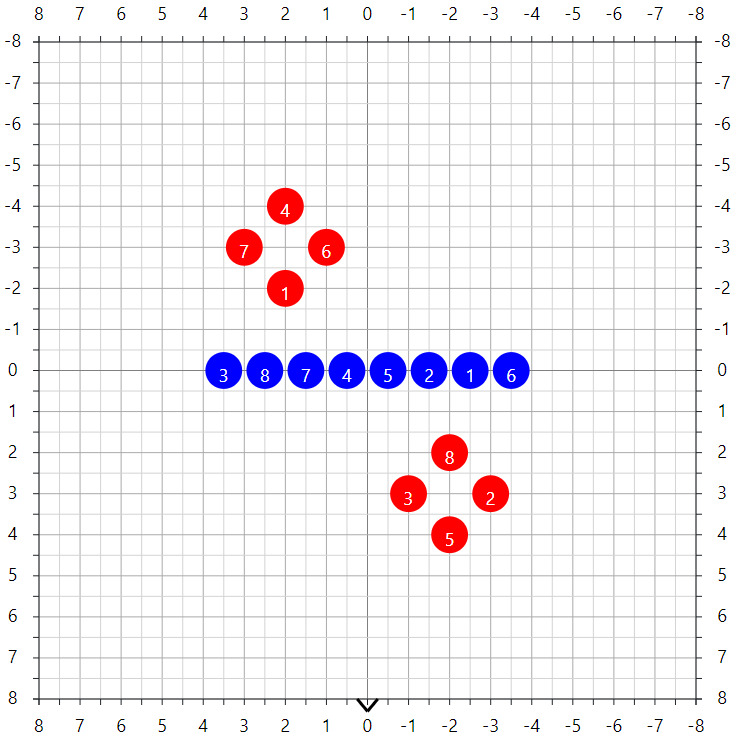
\includegraphics[height=4.5cm]{graphics/definiertes_Bild.png}
    \caption{Definiertes Bild}
    \label{fig:tanzfläche_choreo}
  \end{subfigure}
  \begin{subfigure}{.5\textwidth}
    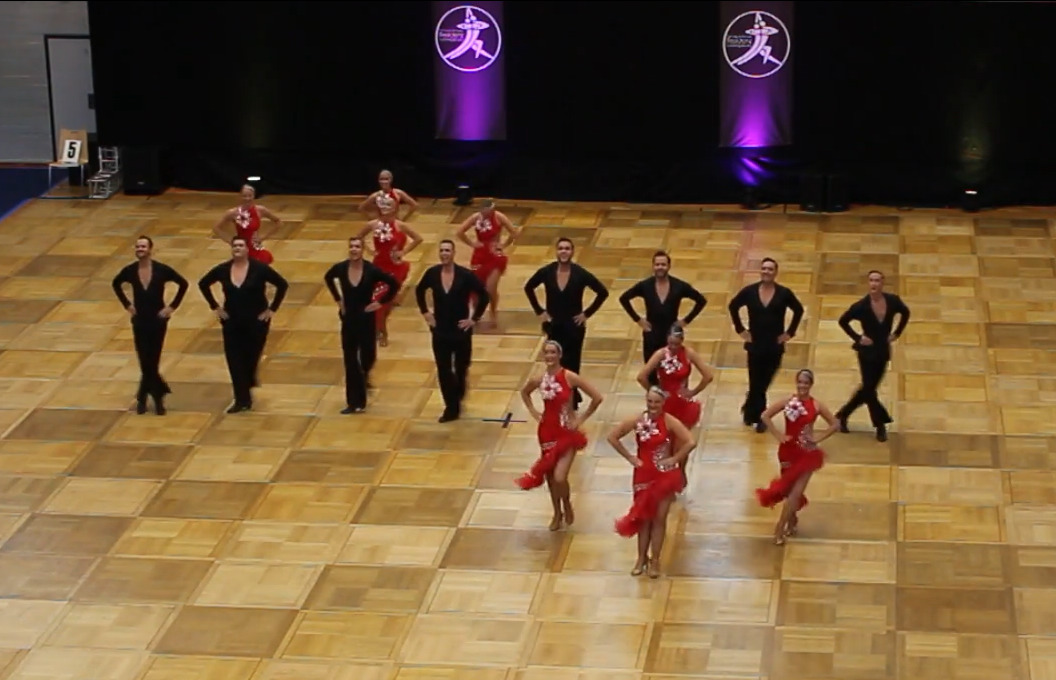
\includegraphics[height=4.5cm]{graphics/getanztes_bild.png}
    \caption{Getanztes Bild}
  \end{subfigure}
  \caption{Vergleich definiertes und getanztes Bild}
  \label{fig:def_bild}
\end{figure}


\subsection{Bewertungskriterien \label{chp:bewertungskriterien}}
Für die Bewertung einer Formationsdarbietung gibt es Wertungsrichtlinien des DTV für Formationswettbewerbe \cite{wertungsrichtlinien}.
Dabei werden Formationen durch Punktevergabe in vier gleichwertige Wertungsgebiete unterteilt: \textit{Musik}, \textit{Tänzerische Leistung}, \textit{Ausführung der Choreographie} und \textit{Durchgängigkeit und Charakteristik}.
Teile der Formation, wie Ein- und Ausmarsch, Erscheinungsbild der Tänzer und Audioqualität der Musik werden nicht bewertet.
Dabei werden je Wertungsgebiet Punkte auf einer Skala von eins bis zehn in einer Wertungstabelle verteilt und summiert.

Im Rahmen der ästhetischen Analyse wird zuerst die \textit{musikalische Dimension} untersucht.
Dabei wird geprüft, ob die Bewegungen ohne Berücksichtigung von Schwierigkeitsgrad, Takt und Grundrhythmus sowie emotionalen und stilistischen Nuancen der Musik ausdrucksstark sind.
Es wird also darauf geachtet, ob der ausgewählte Tanz zur Musik passt.

Das nächste Wertungsgebiet, die \textit{Tänzerische Leistung}, bewertet die Bewegungsqualität, die Anpassung an die Musik und Choreographie, sowie die Gleichheit und Balance aller paare.
Es wird genau darauf geachtet, ob die Übergänge tänzerisch anspruchsvoll sind und eine gleiche Schrittlänge aufweisen, und nicht gegangen oder gelaufen werden.

Als nächstes wird die Aufmerksamkeit auf die \textit{Ausführung der Choreographie} gerichtet.
Hierbei wird geprüft, wie präzise die Paare die Choreografie tanzen.
Kriterien sind, ob geometrische Formen perfekt dargestellt werden, also ob Geraden keine Krümmung aufweisen, Kreise nicht ellyptisch wirken und Symmetrie, beziehungsweise gewollte Asymmetrie korrekt dargestellt wird. Zusätzlich wird die Flächenausnutzung, sowie die Zentrierung zur Mitte betrachtet. Dieses Wertungsgebiet berücksichtigt die Schwierigkeit bei der Bewertung. Im Folgenden werden einige Beispiele für schwierige und weniger schwierige Bewegungen aufgeführt:
\begin{itemize}
  \item Diagonale Linien sind schwieriger als waagerechte oder Senkrechte Linien
  \item Richtungswechsel sind schwieriger als gleichbleibende Richtungen
  \item Je mehr Paare in einem Bild verdeckt zu den Wertungsrichtern stehen, desto schwieriger, da hier Synchronität besonders auffällig
  \item Übergänge mit Rythmuswechsel sind schwieriger als normale Übergänge
\end{itemize}
Die Wahl einer höheren Schwierigkeitsstufe ist für den Erhalt der vollen Punktzahl unerlässlich, birgt jedoch auch ein höheres Risiko.

Die Umsetzung der Choreographie hat einen direkten Einfluss auf die \textit{Durchgängigkeit und die Charakteristik}, das vierte und letzte Wertungsgebiet.
In diesem wird die Umsetzung der Musik und Bilder in Figuren objektiv betrachtet.
Des Weiteren auch die Wechsel zwischen Musik, Tempo und Bildern bewertet und wie gut die Formation dabei geschlossen agiert.
Unter Geschlossenheit versteht man in diesem kontext, wie gut die Tänzerinnen und Tänzer als Einheit agieren.

\section{Algorithmische Grundlagen}
Dieses Kapitel enthält eine für diese Arbeit relevante Sammlung an theoretischen und algorithmischen Grundlagen. Die genaue Verwendung wird in Kapitel 6 bei der Beschreibung der Implementierung näher erläutert.
\subsection{Perspektivische Transformation}
In diesem Abschnitt wird die perspektivische Transformation, eine grundlegende Technik der Computergrafik und Bildverarbeitung, formal erläutert. Die perspektivische Transformation spielt eine entscheidende Rolle bei der Umwandlung von 3D-Szenen in 2D-Bilder und ist in verschiedenen Anwendungsgebieten, einschließlich Computer Vision, von großer Bedeutung. Ein möglicher Algorithmus ist der im Framework OpenCV enthaltene \textit{getPerspectiveTransform}-Algorithmus \cite{src_persp_trans}.

Ziel ist es, eine Liste von Eingangspunkten auf eine Liste von Ausgangspunkten zu transformieren. Im Allgemeinen kann eine perspektivische Transformation folgendermaßen ausgedrückt werden:

\begin{equation}
  \begin{pmatrix} x_i'\\ y_i'\\ 1\end{pmatrix}=\begin{pmatrix}
    a_1 & a_2 & b_1 \\
    a_3 & a_4 & b_2 \\
    c_1 & c_2 & 1
  \end{pmatrix}\cdot\begin{pmatrix}
    x_i \\y_i\\1
  \end{pmatrix}
\end{equation}

Dabei beschreibt $\begin{pmatrix}
    a_1 & a_2 \\
    a_3 & a_4
  \end{pmatrix}$ die Transformationen, $\begin{pmatrix}
    b_1 \\
    b_2
  \end{pmatrix}$ die Translation und $\begin{pmatrix}
    c_1 & c_2
  \end{pmatrix}$ die Projektion.

Wendet man nun die Transformation auf die vier Punkte an, erhält man nach perspektivischer Division die folgenden Gleichungen
\begin{equation}
  x_i'=\frac{a_1\cdot x_i+a_2\cdot y_i+b_1}{c_1\cdot x_i+c_2\cdot y_i +1}\\\forall i\in\{1,2,3,4\}
\end{equation}
\begin{equation}
  y_i'=\frac{a_3\cdot x_i+a_4\cdot y_i+b_2}{c_1\cdot x_i+c_2\cdot y_i +1}\\\forall i\in\{1,2,3,4\}
\end{equation}
Durch Auflösen der Brüche und der Verteilung von $x_i'$ und $y_i'$ erhält man folgende Gleichungen
\begin{equation}
  c_1\cdot x_i\cdot x_i'+c_2\cdot y_i\cdot y_i'+x'i=a_1\cdot x_i+a_2\cdot y_i+b_1\\\forall i\in\{1,2,3,4\}
\end{equation}
\begin{equation}
  c_1\cdot x_i\cdot x_i'+c_2\cdot y_i\cdot y_i'+x_i'=a_3\cdot x_i+a_4\cdot y_i+b_1\\\forall i\in\{1,2,3,4\}
\end{equation}
Bringt man nun alle Unbekannte auf eine Seite, erhält man folgende acht Gleichungen:
\begin{equation}
  a_1\cdot x_i+a_2\cdot y_i+b_1-c_1\cdot x_i\cdot x_i'-c_2\cdot y_i\cdot y_i'=x'i\\\forall i\in\{1,2,3,4\}
\end{equation}
\begin{equation}
  a_3\cdot x_i+a_4\cdot y_i+b_1-c_1\cdot x_i\cdot x_i'-c_2\cdot y_i\cdot y_i'=x'i\\\forall i\in\{1,2,3,4\}
\end{equation}
Dieses Gleichungssystem ist lösbar, denn acht Unbekannte $a_1$, $a_2$, $a_3$, $a_4$, $c_1$, $c_2$, $b_1$ und $b_2$ lassen sich in einem Gleichungssystem mit acht Gleichungen lösen.


% \begin{equation}

% \end{equation}

% \begin{Listing}
%   \begin{lstlisting}[language=python]
%   \end{lstlisting}
%   \caption{Perspektivische Transformation}
%   \label{perspectiveTransform}
% \end{Listing}

\subsection{Lineare Interpolation}
In diesem Abschnitt wird die lineare Interpolation, eine grundlegende Methode in der numerischen Analyse und Datenarbeit formal erläutert. Bei der linearen Interpolation handelt es sich um ein mathematisches Verfahren zur Schätzung von Zwischenwerten basierent auf bekannten Datenpunkten. Diese Interpolation zwischen den Punten $(x_0,y_0)$ und $(x_1,y_1)$ lässt sich formal wie folgt ausdrücken:

\begin{equation}
  \frac{y-y_0}{x-x_0}=\frac{y_1-y_0}{x_1-x_0}
\end{equation}
Um für einen x-Wert den y-Wert zu berechnen muss die Gleichung folgendermaßen gelöst werden:
\begin{equation}
  y=\frac{y_0(x_1-x)+y_2(x-x_0)}{x_1-x_0}
\end{equation}


\section{Analyse von Trajektorien im Sport}


\chapter{Methodik \label{chp:methodik}}
Dieses Kapitel erläutert die Methodik, die im Rahmen dieser Arbeit angewandt wurde. Naheliegend ist es, einen vorhandenen Ansatz als Orientierung für die Vorgehensweise in der Arbeit zu nutzen. Dafür wird der nutzerorientierte Ansatz aus der Arbeit von Sedlmair et. al. \cite{sedlmair_design_2012} verwendet, welche sich damit befasst, eine Entwicklung mithilfe einer Designstudie zu unterstützen. Folglich wird die Theorie und Durchführung einer problemorientierten Forschung erläutert und im Anschluss die Anwendung des Konzepts auf die vorliegende Arbeit dargelegt.
\section{Vorgehensmodell}

Beschrieben wird eine Designstudie als \enquote{ein Projekt, in dem Visualisierungsforscher ein spezifisches reales Problem analysieren, mit dem Fachleute konfrontiert sind, ein Visualisierungssystem entwerfen, das die Lösung dieses Problems unterstützt, das Design validieren, über die gewonnenen Erkenntnisse nachdenken, um die Richtlinien für das Visualisierungsdesign zu verfeinern} (übersetzte Definition aus \cite{sedlmair_design_2012}).

Die Durchführung einer Designstudie mittels dem neun-stufigen Modell kann zu drei verschiedenen Ergebnissen führen: \textit{Problemcharakterisierung und -abstraktion}, \textit{validierte Visualisierungslösung} oder \textit{Reflektion über das Design und Vergleich mit anderer Forschung}. Das neun-stufige Vorgehensmodell kann in Abbildung \ref{fig:vorgehensmodell} eingesehen werden und wird im Folgenden in seinen Stufen beschrieben und auf diese Arbeit übertragen.

\begin{figure}
  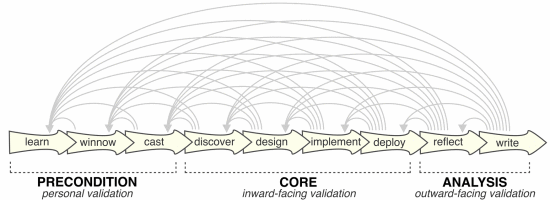
\includegraphics[width=\textwidth]{graphics/vorgehensmodell.png}
  \caption{Vorgehensmodell nach Sedlmair et. al. \cite{sedlmair_design_2012}}
  \label{fig:vorgehensmodell}
\end{figure}

Die Stufen sind in drei Kategorien verteilt, der \textit{Vorbereitunsphase}, der \textit{Kernphase}, also die wichtigsten Schritte bei der Durchführung der Studie und der \textit{Analysephase}, also die Auswertung der Studie, sowie das ermitteln von Erkenntnissen. Der allgemeine Aufbau der Kategorien und der enthaltenen Stufen ist linear, dennoch gibt es häufig Fälle, in denen Stufen übersprungen, oder nach Erkenntnis neuer Informationen wieder eine oder mehrere Stufen zurückgesprungen werden müssen. Auch sind Überschneidungen durchaus möglich. Dennoch sollte man mit übermäßigem Springen vorsichtig sein, denn beispielsweise eine Entwicklung eines Prototypen vor der Analyse der Anforderungen aller Stakeholder kann das Projekt initial in eine völlig falsche Richtung lenken. Für diese Arbeit kann dieses Modell jedoch nicht in vollem Unfang eingehalten werden, denn es werden beispielsweise für den Deploy oder das Schreiben eine Zeitzuweisung von mehreren Monaten vorgesehen, was bei einer halbjährigen Arbeit nicht möglich ist. Durch die gesammelten Erfahrungen in diesem Projekt erschließt sich eine großzügige Zeitzuweisung dennoch als äußerst sinnvoll.

Die Vorbereitungsphasen \textit{Learn}, \textit{Winnow} und \textit{Cast} konzentrieren sich darauf, wichtige Fragen und Erkenntnisse über die Domäne und der verwendeten Technologie vor dem Start der eigentlichen Implementierung anzueignen.

In der \textit{Learn}-Phase geht es darum, ein solides Verständnis für Visualisierung und Entwurfsrichtlinien mithilfe von Literatur und Forschung zu erlangen. Darunter werden in dieser Phase möglichen Techniken und Bibliotheken, sowie Bewertungsmethoden behandelt. Hierfür wurde im Rahmen der vorliegenden Arbeit ein vergangenes Studienprojekt zur Verfügung gestellt und eine ausführliche Beratung durch die Betreuer angeboten. Für die Vorgehensweise wurde die Arbeit von Sedlmair et al. \cite{sedlmair_design_2012} herangezogen.

Dieses angeeignete Wissen hilft in der \textit{Winnow}-Phase, geeignete Experten für die Durchführung des Projekts zu finden. Dieser Prozess erfordert sorgfältige Auswahl aus einer breiten Palette möglicher Interessenten und ist langwierig. Letztendlich müssen die Interessen der Experten und Forscher klar übereinstimmen. Aufgrund beschränkter Zeit wurden die Experten im Rahmen dieser Arbeit ausgewählt. Etwa zur Halbzeit fand ein erstes Treffen statt. Die Experten sind Tanzlehrer einer Formationsmannschaft, die im vergangenen Studienprojekt bereits gute Erfahrungen gesammelt haben und wertvolle Einwände zur Umsetzung des Prototyps dieser Arbeit beisteuern konnten.

Den Abschluss der Vorbereitunsphase bildet die \textit{Cast}-Phase, in der die Rollen der Kollaboratoren definiert werden. Dabei wird zwischen die entscheidenden Rollen unterschieden, dem Frontline-Analyst, der als Endnutzer die eigentliche Datenanalyse und Anwendung des Tools durchführt, und Gatekeeper, eine Person mit der Befugnis, das Projekt zu genehmigen oder zu blockieren, sowie die weitere Administration. Konnektoren sind Personen, die den Forscher mit anderen interessanten Personen, meist Frontline-Analysten zusammenbringen. Die Domänenexperten sind in diesem Fall die Frontline-Analysten, die das entwickelte Analysetool in den Trainingsalltag einbinden möchten. Die Betreuer haben sowohl die Rolle der Gatekeeper mit dem Professor eingenommen, jedoch auch als Konnektoren gewirkt, um den Forscher mit den Domänenexperten in Verbindung zu bringen.

Nach der Vorbereitungsphase beginnt nun der eigentliche Kern der Designstudie, in der das gesammelte Wissen in die Entwicklung eines Designvorschlags einfließen.


\section{Durchgeführte Designstudie}



\subsection{Erstes Interview: Anforderungsanalyse}
Das Interview fand in etwa drei Monate nach Projektbeginn statt. Ziel war es, das erarbeitete Wissen über die Domäne zu verifizieren und
\subsection{Zweites Interview: Bewertung}
\section{Durchgeführte Studie am Prototypen}

\chapter{Konzept \label{chp:konzept}}
Die Konzeptentwicklung ist ein entscheidender Schritt im Entwicklungsprozess, da sie die Grundlage für die Gestaltung des Prototyps legt. In dieser Phase werden grundlegende Überlegungen und Ideen entwickelt, um die Richtung und den Fokus des Prototyps festzulegen. Im Zentrum stehen die Identifizierung von Schlüsselmerkmalen und -funktionen, für die verschiedene Ansätze und Lösungen in Betracht gezogen werden, um die bestmögliche Umsetzung der gestellten Anforderungen zu erreichen. Dieser kreative Prozess läuft parallel zur Anforderungsanalyse und Recherche und nutzt die gewonnenen Erkenntnisse, um das Konzept iterativ zu verfeinern und an die spezifischen Anforderungen anzupassen.

Parallel hierzu spielen auch technische Aspekte eine entscheidende Rolle. Die Auswahl der richtigen Technologien und Plattformen haben neben der Realisierbarkeit auch einen Einfluss Verfügbarkeit. Daher werden während der Konzeptentwicklung auch technologische Überlegungen angestellt, um sicherzustellen, dass der Prototyp sowohl innovativ als auch praktisch umsetzbar ist. Nach sorgfältiger Abwägung der Möglichkeiten wurde sich auf das Zusammenspiel mehrerer Technologien geeinigt. An erster Stelle steht OpenCV, ein Framework, das sich für transformative Operationen auf dem Datensatz gut eignet. Zur Realisierung des Prototyps wurde React als Framework ausgewählt, weil damit eine interaktive Benutzeroberfläche mit Browserzugriff umgesetzt werden konnte. Schließlich wurde die renommierte und vielseitig genutzte Bibliothek D3 für die dynamische Erstellung interaktiver Datenvisualisierungen verwendet. Genauer darauf wird in Kapitel \ref{chp:implementierung} eingegangen, in dem die Implementierung detailliert behandelt wird.

Nachdem die grundlegenden Konzepte feststehen, folgt die nächste wichtige Phase der Konzeptentwicklung: das System in verschiedene Komponenten zu gliedern. Diese Strukturierung ermöglicht eine detaillierte Analyse einzelner Funktionseinheiten und erleichtert die spätere Entwicklung sowie die Anpassung des Prototyps im Laufe der Zeit. Üblicherweise wird das System nach funktionalen und logischen Gesichtspunkten in Komponenten unterteilt. Dieser Ansatz reduziert die Komplexität des Gesamtsystems und schafft eine klare Struktur. Dabei werden die spezifischen Aufgaben und Verantwortlichkeiten jeder einzelnen Komponente optimiert.

In diesem Abschnitt werden die Systemkomponenten im Detail betrachtet. Es werden ihre Grundüberlegungen und Funktionalitäten beschrieben sowie eventuelle Veränderungen im Laufe der Zeit. Ein Einblick in die Entwicklungsgeschichte der einzelnen Komponenten ist entscheidend, um die Entscheidungsprozesse und Iterationen während des Entwicklungsprozesses nachvollziehen zu können.

\section{Visualisierung der Tanzfläche}
Für die graphische Visualisierung der Tanzfläche wird auf der bisherigen Visualisierung der Choreographie aufgebaut, welche bereits in Abbildung \ref{fig:tanzfläche_choreo} angegeben ist. Dies hat den Vorteil, dass die einzelnen Tänzerinnen und Tänzer auf einer Meterskala dargestellt werden können, um eine Verbindung zur Realität zu erhalten. Zu dieser Skala sollen folgende Funktionen hinzugefügt werden:
% \begin{itemize}
%   \item Darstellung der Abweichung eines Tänzers zum in der Choreographie definierten Bild
%   \item Auswahl von Tänzern und Tänzerinnen in den Fokus
%   \item Visualisierung der Trajektorien zwischen mehreren Bildern in der Choreographie
% \end{itemize}
\paragraph{Darstellung der Abweichung eines Tänzers zum in der Choreographie definierten Bild}
Die Visualisierung der Abweichung eines Tänzers von der vorgegebenen Choreographie ist für die Beurteilung der Qualität einer Tanzperformance von zentraler Bedeutung. Dabei können verschiedene Metriken berücksichtigt werden. Die Implementierung dieser Funktion ermöglicht es, einzelne Tänzerinnen und Tänzer hervorzuheben, die signifikant von der Choreographie abweichen. Dadurch können gezielte Verbesserungen vorgeschlagen und eine präzisere Anpassung der Tanzbewegungen erreicht werden.
\paragraph{Auswahl von Tänzern und Tänzerinnen in den Fokus}
\paragraph{Visualisierung der Trajektorien zwischen mehreren Bildern in der Choreographie}
\section{Einbinden des Videos}
Um ein besseres Verständnis über das im Koordinatensystem visualisierte Frame aus der Choreographie zu erhalten, soll das Originalvideo in den Prototypen miteingebaut werden. Eine hilfreiche Funktionalität ist, im Video die Boundingbox der auf der Visualisierung der Tanzfläche ausgewählten Tänzer und Tänzerinnen anzuzeigen. Somit kann von der abstrakten Darstellung eine Verknüpfung zur Realität erstellt werden.
\section{Interaktiver Zeitleiste}


% \section{Skizzen}
\begin{figure}
  \centering
  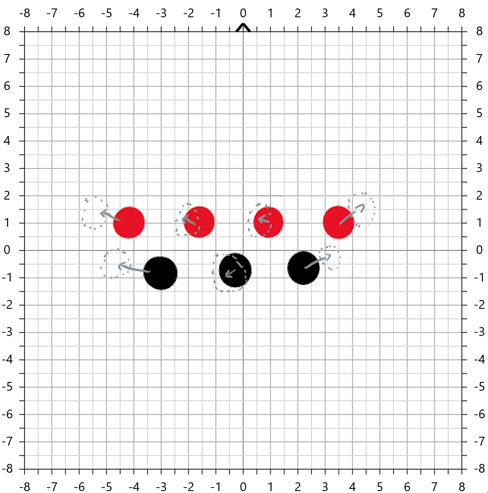
\includegraphics[width=0.6\textwidth]{graphics/vorschlag_positionsabweichung_koordinatensystem.png}
  \caption{Vorschlag Darstellung der Abweichung vom definierten Bild}
  \label{fig:tanzfläche}
\end{figure}
\begin{figure}
  \centering
  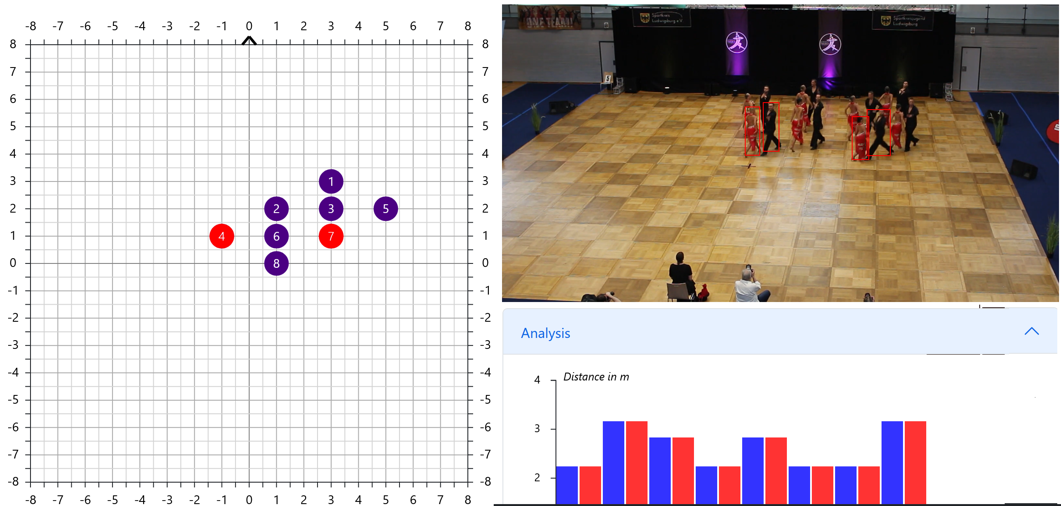
\includegraphics[width=\textwidth]{graphics/vorschlag_videoeinbindung_mit_bbox.png}
  \caption{Vorschlag Videoeinbindung mit Anzeigen von BoundingBoxen}
  \label{fig:video}
\end{figure}
\begin{figure}
  \centering
  
\includegraphics[width=\textwidth]{graphics/vorschlag_timeline.png}
  \caption{Vorschlag Timeline mit Diagramm}
  \label{fig:timeline}
\end{figure}
% \section{Gedankliches Konzept}
% \section{Umgesetzt/ nicht umgesetzt}

\chapter{Implementierung \label{chp:implementierung}}
\section{Verwendete Technologien}
Der Prototyp wurde als webbasierte Single-page application mithilfe von TypeScript entwickelt und basiert auf einem früheren privaten Prototypen aus einem früheren Projekt, der weiterentwickelt wurde. Dieses Konzept wurde gewählt, denn SPAs ermöglichen eine native App-ähnliche Benutzererfahrung im Web.
\subsection{OpenCV}
Die Open Source Computer Vision Library (OpenCV) ist eine leistungsstarke Softwarebibliothek für Computer Vision und maschinelles Lernen. Die Bibliothek verfügt über mehr als 2500 optimierte Algorithmen, die sich ideal für Aufgaben im Bereich maschinelles Lernen und Bildverarbeitung eignen \cite{opencv2023about}. Eine entscheidende Funktion dieser Bibliothek, die für dieses Projekt von großer Bedeutung ist, beinhaltet das Arbeiten auf Bildern mit Skalierungen, Translationen und andere Transformationen. Hierfür wird ein Video in Form eines VideoCapture-Objekts eingelesen. Dieses Objekt repräsentiert eine Sequenz von Bildern, die dann schrittweise durchlaufen werden können, um gewünschte Transformationen anzuwenden.


\subsection{React}

React ist eine ursprünglich von  Facebook, Inc. (heute Meta Platforms, Inc.) entwickelte, nach einem Jahr frei zugänglich gemachte, JavaScript Bibliothek für das Erstellen von Benutzeroberflächen. Es wurde entwickelt, um große Anwendungen mit veränderlichen Daten zu implementieren und stellt den \glqq View\grqq-Teil des Model-View-Controller-Entwicklungsparadigmas bereit \cite{krill2023react}. Dabei handelt es sich um einen Ansatz, die Anwendung von der Benutzeroberfläche zu trennen \cite{deacon-model-view-controller2009}. Dieses Paradigma setzt sich aus drei wesentlichen Komponenten zusammen: dem Datenbereich (Model), der Steuerungslogik (Controller) und der von React erstellten Benutzeroberfläche (View), wie in Abbildung \ref{fig:MVCdiag} veranschaulicht.
\begin{figure}
  \centering
  \begin{tikzpicture}
    % Erstes Oval
    \node[draw, ellipse] (ctrl) at (0,0) {Controller};
    % Zweites Oval
    \node[draw, ellipse] (view) at (3,0) {View};
    % Drittes Oval
    \node[draw, ellipse] (model) at (1.5,2.5) {Model};

    % Anpassung der Pfeillänge
    \draw[->, shorten >= 3pt, shorten <= 3pt,] (ctrl) -- (view);
    \draw[->, shorten >= 3pt, shorten <= 3pt] (view) -- (model);
    \draw[->, shorten >= 3pt, shorten <= 3pt] (ctrl) -- (model);
    \draw[->, shorten >= 3pt, shorten <= 3pt, dotted] (model) to [out=-30, in=90] (view);

  \end{tikzpicture}
  \caption{Model-View-Controller \cite{inbook}}
  \label{fig:MVCdiag}

\end{figure}



React ermöglicht es, die Oberfläche in einzelne Teile nahmens Komponenten zu zerlegen, die dann kombiniert werden können \cite{react2023}. Solche Komponenten können so klein wie ein simpler Button oder so groß wie eine ganze Webseite sein. Jede Komponente besitzt ihren eigenen Zustand, und wenn sich dieser Zustand ändert, wird auch der Zustand der gesamten App geändert. Im Beispiel in Listing \ref{lst:MyButton} sehen Sie eine einfache React-Komponente, welche einen einfachen Button erstellt. Diese Komponente wird in Listing \ref{lst:MyApp} in eine weitere Komponente namens MyApp verschachelt.

\lstinputlisting[language=Java,label=lst:MyButton,caption={Simple Button Component},float]{code/MyButton.tsx}
\lstinputlisting[language=Java,label=lst:MyApp,caption={Simple React App},float]{code/MyApp.tsx}


Es hat sich als Standard etabliert, Komponenten in der Markup-Syntax TSX (oder JSX in JavaScript) zu schreiben zur Vereinfachung. Dadurch wird das Einbetten von Code in das zurückgegebene Element ermöglicht. Diese Syntax ist strenger als HTML und erlaubt nur das Zurückgeben eines einzelnen TSX-Tags pro Komponente, wodurch jede Komponente ein einzelnes Element darstellt.

React arbeitet nach dem Prinzip der Reconciliation \cite{virtualDOM}. Dabei wird eine virtuelle Darstellung der Anwendung im Speicher gehalten und durch die ReactDOM-Bibliothek mit dem tatsächlichen DOM synchronisiert. Durch diesen Ansatz wird die deklarative API von React ermöglicht. Man teilt React mit, in welchem Zustand die Benutzeroberfläche sein sollte, und React stellt sicher, dass das DOM diesem Zustand entspricht. Dadurch werden die Manipulation von Attributen, die Behandlung von Ereignissen und die manuelle Aktualisierung des DOMs abstrahiert, die der Entwickler selbst bei der Entwicklung der Anwendung durchführen müsste.

\paragraph{Document Object Model}

Das wichtige Rückgrad einer modernen Webanwendung für Manipulation und Darstellung ist das Document Object Model. Durch das dieses wird ein HTML-Dokument in Form eines logischen Baums dargestellt. Dabei endet jeder Zweig in einem Knoten, welcher Objekte enthält. Dieser Baum ermöglicht einen programmatischen Zugriff, um den Stil oder Inhalt des Dokuments zu ändern.






\subsection{D3}
\subsection{Zusammenspiel React und D3}
In der Welt der Webentwicklung stoßen Entwickler häufig auf Herausforderungen, wenn sie React und D3.js, zwei mächtige Bibliotheken für die Benutzeroberflächengestaltung und Datenvisualisierung, miteinander kombinieren möchten.
Ein grundlegendes Problem ergibt sich aus der Art und Weise, wie React und D3 mit dem Document Object Model (DOM) interagieren.

React verwaltet den DOM effizient durch die Verwendung des Virtual DOM und aktualisiert ihn bedarfsorientiert. Im Gegensatz dazu arbeitet D3 direkt mit dem DOM und manipuliert es, um Daten zu visualisieren. Diese unterschiedlichen Ansätze können zu Konflikten führen, wenn beide Bibliotheken gleichzeitig versuchen, das DOM zu ändern. Unvorsichtige Integrationen können zu unerwartetem Verhalten und Fehlern führen. Eine mögliche Lösung für dieses Problem besteht darin, eine React-Komponente zu erstellen, welche das SVG-Element enthält, in dem die D3-Visualisierung erstellt werden soll. Dabei wird auf einer Referenz auf ein SVG-Element im DOM gearbeitet und mittels der useEffect-Funktion eine Visualisierung angewendet.

\section{Transformation}
\lstinputlisting[language=Python,label=lst:n_point_transformation,caption={N\_Points\_Transformation},float]{code/n_points_transformation.py}
\subsection{RANSAC}

\section{Datenvorverarbeitung \label{chp:datenvorbereitung}}
\section{Prototyp}

\chapter{Evaluation \label{chp:evaluation}}
\section{Studie}
\subsection{Studienaufbau}
\subsection{Teilnehmer}
\subsection{Forschungsfragen}
\subsection{Evaluationsmethoden}
\section{Resultate und Interpretation}
\section{Einschränkungen}
\section{Schlussfolgerung}


\chapter{Probleme und Herausforderungen \label{chp:probleme}}
Im Fokus dieses Kapitels steht die Auseinandersetzung von identifizierten Problemen und Herausforderungen. Dabei werden nicht nur die Schwierigkeiten beleuchtet, die bei der Erstellung des Prototypen auftraten, sondern auch die Einschränkungen des Prototyps untersucht, die Aufgrund von verschiedenen Faktoren und Annahmen auftreten.
\section{Extraktion mittels Computer Vision Methoden}

Der bisherige Ansatz, die Positionen der Tänzerinnen und Tänzer aus dem Videomaterial zu analysieren, war zwar für die Entwicklung eines Prototyps ausreichend, ist aber in der Realität, d.h. im regulären Trainingsalltag, nicht praktikabel. Denn das in Kapitel \ref{chp:datenvorbereitung} beschriebene Extraktionsverfahren erfordert die framegenaue Annotation von Bounding Boxes im Videomaterial mittels einer Software. Diese Methode ist jedoch sehr zeitaufwendig, da die Analyse mehrere Stunden bis Tage dauert, wenn sie von einer Person durchgeführt wird. Daher müssen die Trainer entweder viel wertvolle Zeit in die Nachbereitung des Trainings investieren oder teures Personal einstellen, das diese Arbeit übernimmt - beides ist nicht praktikabel.
Im Vorfeld der Entwicklung des Prototyps wurde daher nach alternativen Methoden gesucht. Als besonders vielversprechend erwies sich der Einsatz von softwarebasierten Motion Trackern. Dies hätte den Vorteil, dass die Boundingboxen algorithmisch generiert werden und somit viel Arbeit eingespart werden könnte. In einer idealen Umgebung wäre dieser Ansatz die perfekte Lösung und würde lediglich die Definition der Choreographie sowie eine Videoaufzeichnung der Trainingseinheit erfordern. In der Praxis weist dieser Ansatz jedoch zahlreiche Einschränkungen auf. Dies ist auf eine Reihe von Faktoren zurückzuführen, die im Folgenden diskutiert werden.

Ein Problem liegt in der Hardware der Kamera. Ein Tracker kann nur so gut arbeiten, wie die zur Verfügung stehenden Daten. Das zur Verfügung gestellte Videomaterial hatte eine relativ geringe Auflösung, so dass selbst für das menschliche Auge an manchen Stellen nicht erkennbar war, zu welcher Tänzerin oder zu welchem Tänzer das halb verdeckte Körperteil gehörte. In Kombination mit der gleichen Kleidung, die die Tänzerinnen und Tänzer tragen, nämlich rote Kleider für die Frauen und schwarze Anzüge für die Männer, ist eine Unterscheidung der Tänzerinnen und Tänzer durch den Tracker, insbesondere bei teilweiser oder vollständiger Verdeckung, nicht möglich. Tracker wie Tapnet arbeiten mit Punktverfolgung. Durch die geringe Auflösung und auch durch Rotationen gehen diese Punkte regelmäßig verloren. Dadurch ist der Analyseaufwand noch höher als bei einer manuellen Analyse. Nicht zu vernachlässigen ist auch der Rechenaufwand der Hardware bei der Extraktion der Trajektorien aus dem Video. Hier besteht ein Trade-off zwischen der Laufzeit und dem Rechenaufwand des Algorithmus und der Genauigkeit der extrahierten Trajektorien. Denn selbst mit der heute überdurchschnittlich leistungsfähigen Hardware ist die Analyse mit hoher Genauigkeit sehr zeitaufwendig. Mit diesem Ansatz würde die Zielgruppe einer solchen Software stark eingeschränkt und das System wäre nicht für jedermann nutzbar.

Für diese Probleme gibt es verschiedene Lösungsansätze. Neben der Investition in besseres Equipment kann während des Trainings unterschiedliche Kleidung getragen werden, um die Tänzer farblich zu unterscheiden. Mithilfe von Filtern können dann alle Tänzer bis auf einen ausgeblendet werden, um die genaue Position zu extrahieren. Zusätzlich wäre es hilfreich, eine Kamera über der Tanzfläche zu installieren, um eine Überlappung der Tänzer zu vermeiden. Ansätze wie die Ausstattung des Raumes mit mehreren Kameras oder ein Boden, der die Positionen durch Berührung ermitteln kann, würden den Rahmen dieser Domäne sprengen.

\section{Probleme mit linearer Interpolation}
Eine Lateinformationschoreographie wird durch eine Reihe von Formationsbildern definiert. Aus diesem Grund ergibt sich bei der Implementierung eines Prototyps mit für den Menschen kontinuierlicher Granularität das Problem, dass die Trajektorien in kontinuierlicher Form vorliegen, während die Formationsbilder nur diskret definiert sind. Dies bedeutet, dass die Trajektorie zwischen diesen Bildern undefiniert ist und interpoliert werden muss. Im Rahmen dieser Arbeit wurde die lineare Interpolation als Ansatz zur Lösung des Problems verwendet. Der Vorteil dieser Methode ist, dass sie einfach und ohne großen Rechenaufwand durchgeführt werden kann. Die Problematik dieses Ansatzes geht mit der Definition aus den im Abschnitt \ref{chp:bewertungskriterien} beschriebenen Bewertungskriterien des DTV \cite{wertungsrichtlinien} einher, dass Übergänge tänzerisch anspruchsvoll sein müssen, d.h. eine lineare Interpolation führt oft zu Ungenauigkeiten bei diesen Übergängen.

%TODO bildliches Beispiel%

\section{Zukünftige Forschung}
\section{Kritik von Experten}
\section{Weiterentwicklung Ansatz}

\chapter{Zusammenfassung \label{chp:zusammenfassung}}
\section{Zukünftige Forschung}
\section{Wichtigste Erkenntnisse}
\section{Bedeutung Arbeit für Forschungsfeld}

\printbibliography

% Alle URLs wurden zuletzt am 17.\,03.\,2018 geprüft.
Alle URLs wurden zuletzt am \today \space geprüft.

%\renewcommand{\appendixtocname}{Anhang}
%\renewcommand{\appendixname}{Anhang}
%\renewcommand{\appendixpagename}{Anhang}
\appendix


\pagestyle{empty}
\renewcommand*{\chapterpagestyle}{empty}
\Versicherung
\end{document}
